
% \ref{non-crime-no-timeseries-result}同様に予測結果を示す.

2014年に実際に起った強盗犯罪の発生地点に基づいた実際のリスクマップを
図\ref{fig:non-crime-timeseries-actual-risk}に示す.
DFによるリスクマップを図\ref{fig:non-crime-timeseries-df-risk}に,
CFによるリスクマップを図\ref{fig:non-crime-timeseries-cf-risk}に,
CIによるリスクマップを図\ref{fig:non-crime-timeseries-ci-risk}に
% NEによるリスクマップを図\ref{fig:non-crime-timeseries-ne-risk}に,
% LDによるリスクマップを図\ref{fig:non-crime-timeseries-ld-risk}に,
% GFによるリスクマップを図\ref{fig:non-crime-timeseries-gf-risk}に,
% TGによるリスクマップを図\ref{fig:non-crime-timeseries-tg-risk}に,
% GF+TGによるリスクマップを図\ref{fig:non-crime-timeseries-gf-tg-risk}
示す.
% \ref{non-crime-no-timeseries-result}同様に,
実際のリスクマップと比べて,離散型特徴量(DF)によるリスクマップでは高い空間相関を持つが,
連続型特徴量(CF)と犯罪込み連続型特徴量(CI)によるリスクマップは空間相関が削減された.


% また,
% 4カテゴリーの混同行列を図\ref{fig:non-crime-timeseries-4cm}に,
% 2カテゴリーの混同行列を図\ref{fig:non-crime-timeseries-2cm}に,
% 各モデルによるFP・FNのグリッドセルを
% 図\ref{fig:non-crime-timeseries-df-fnp}から
% 図\ref{fig:non-crime-timeseries-gf-tg-fnp}に示した.

%------------------------------------------
% risk map
%------------------------------------------
\begin{figure}[H]
  \centering % 図を中央寄せにする
  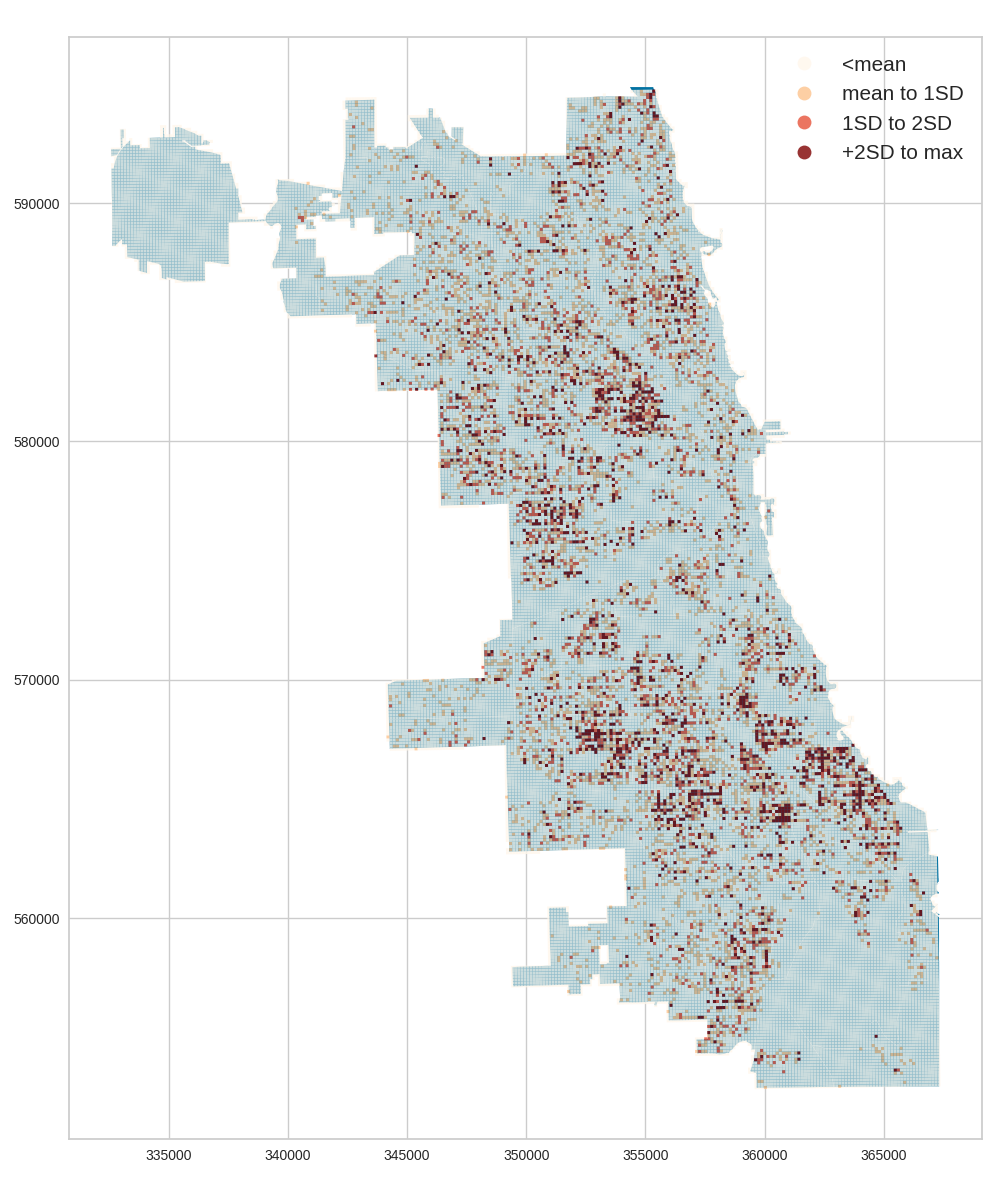
\includegraphics[scale=0.15]{./figures/actual_riskmap.png}
  \caption{実際のリスクマップ}
  \label{fig:non-crime-timeseries-actual-risk}
\end{figure}

\begin{figure}[H]
  \centering % 図を中央寄せにする
  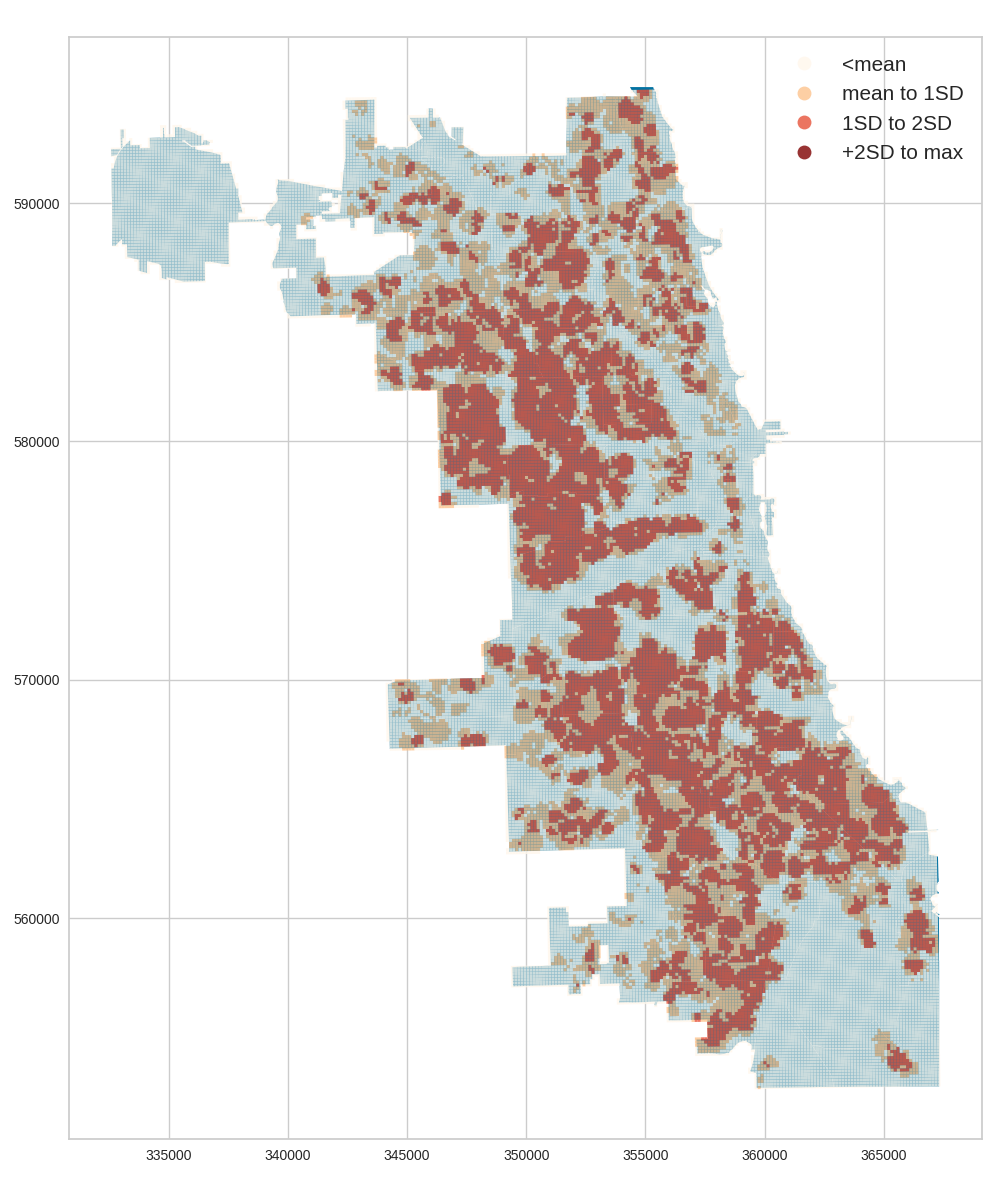
\includegraphics[scale=0.15]{./figures/DF_riskmap.png}
  \caption{DFによるリスクマップ}
  \label{fig:non-crime-timeseries-df-risk}
\end{figure}

\begin{figure}[H]
  \centering % 図を中央寄せにする
  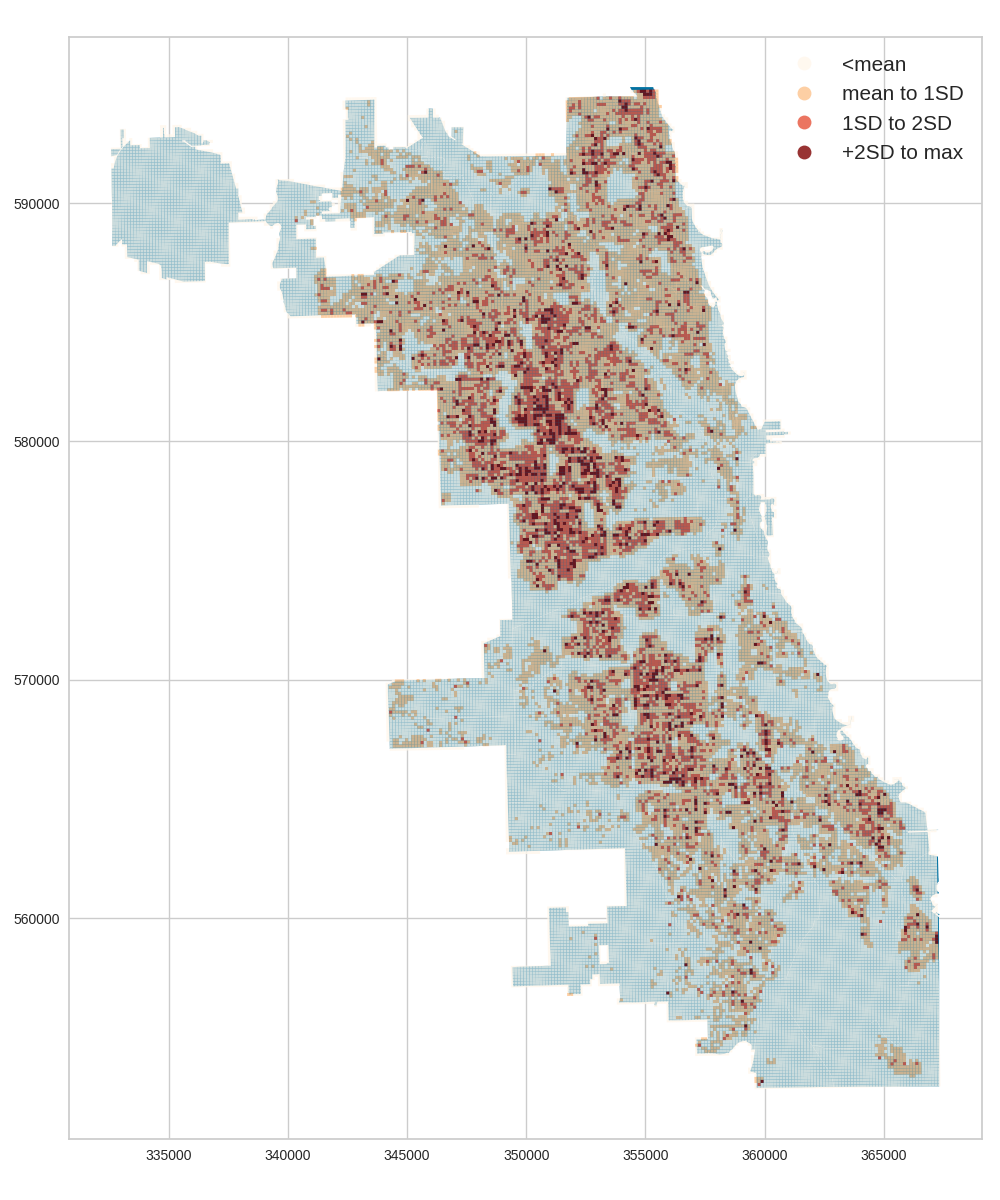
\includegraphics[scale=0.15]{./figures/CF_riskmap.png}
  \caption{CFによるリスクマップ}
  \label{fig:non-crime-timeseries-cf-risk}
\end{figure}

\begin{figure}[H]
  \centering % 図を中央寄せにする
  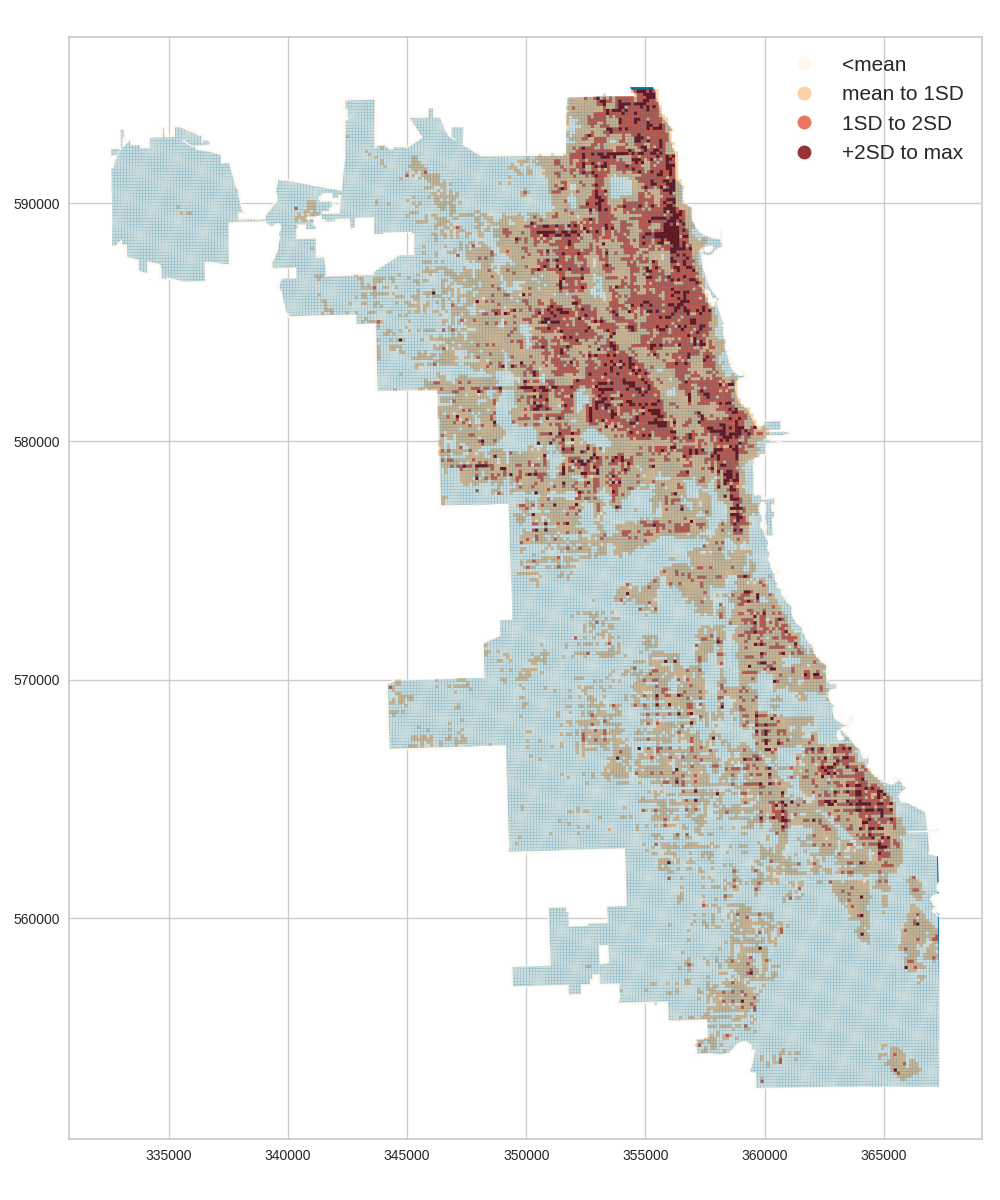
\includegraphics[scale=0.15]{./figures/CI_riskmap.png}
  \caption{CIによるリスクマップ}
  \label{fig:non-crime-timeseries-ci-risk}
\end{figure}

% \begin{figure}
%   \centering % 図を中央寄せにする
%   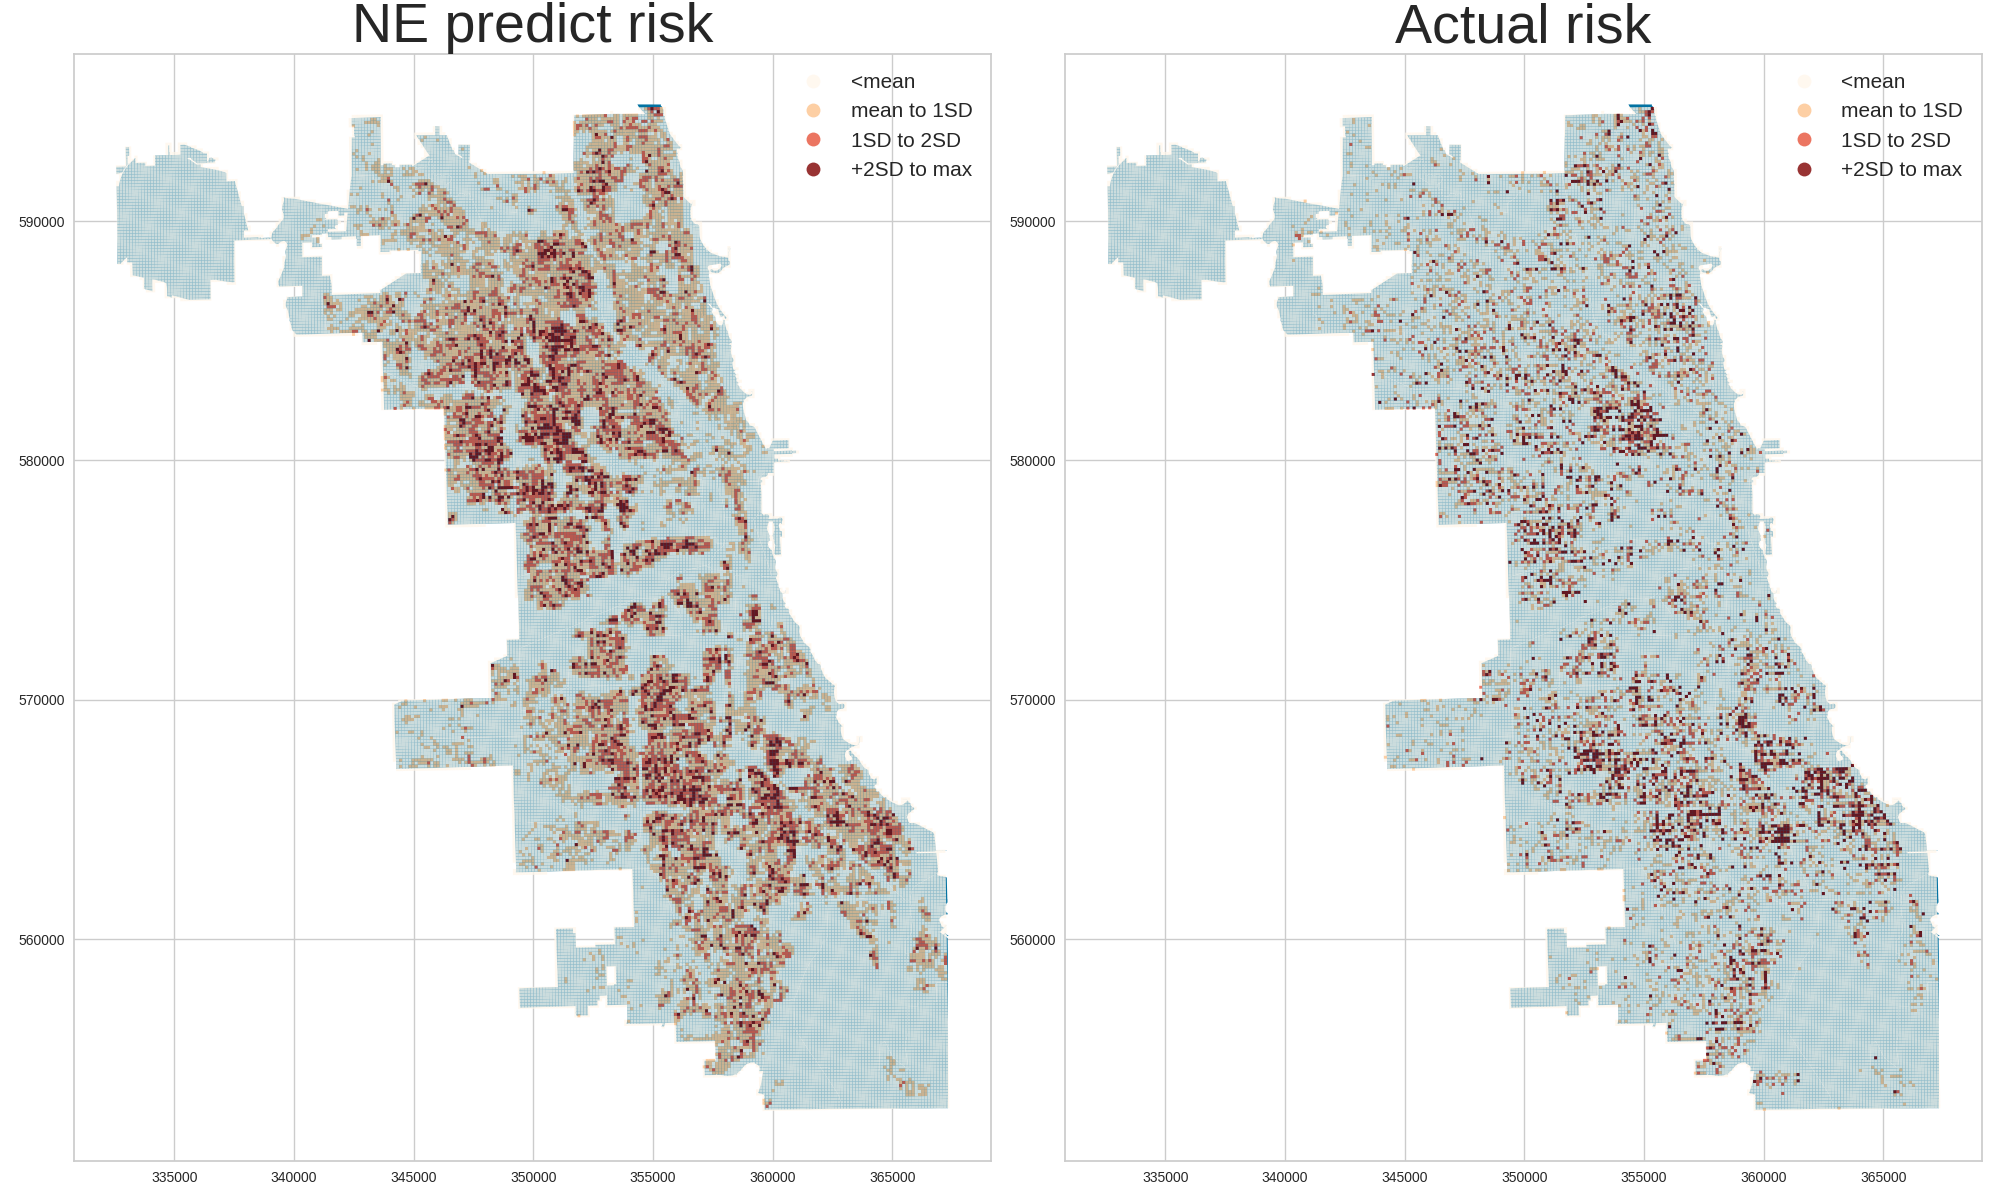
\includegraphics[scale=0.25]{./non-crime-timeseries-fig/NE_riskmap.png}
%   \caption{左:NEによるリスクマップ 右:実際のリスクマップ}
%   \label{fig:non-crime-timeseries-ne-risk}
% \end{figure}

% \begin{figure}
%   \centering % 図を中央寄せにする
%   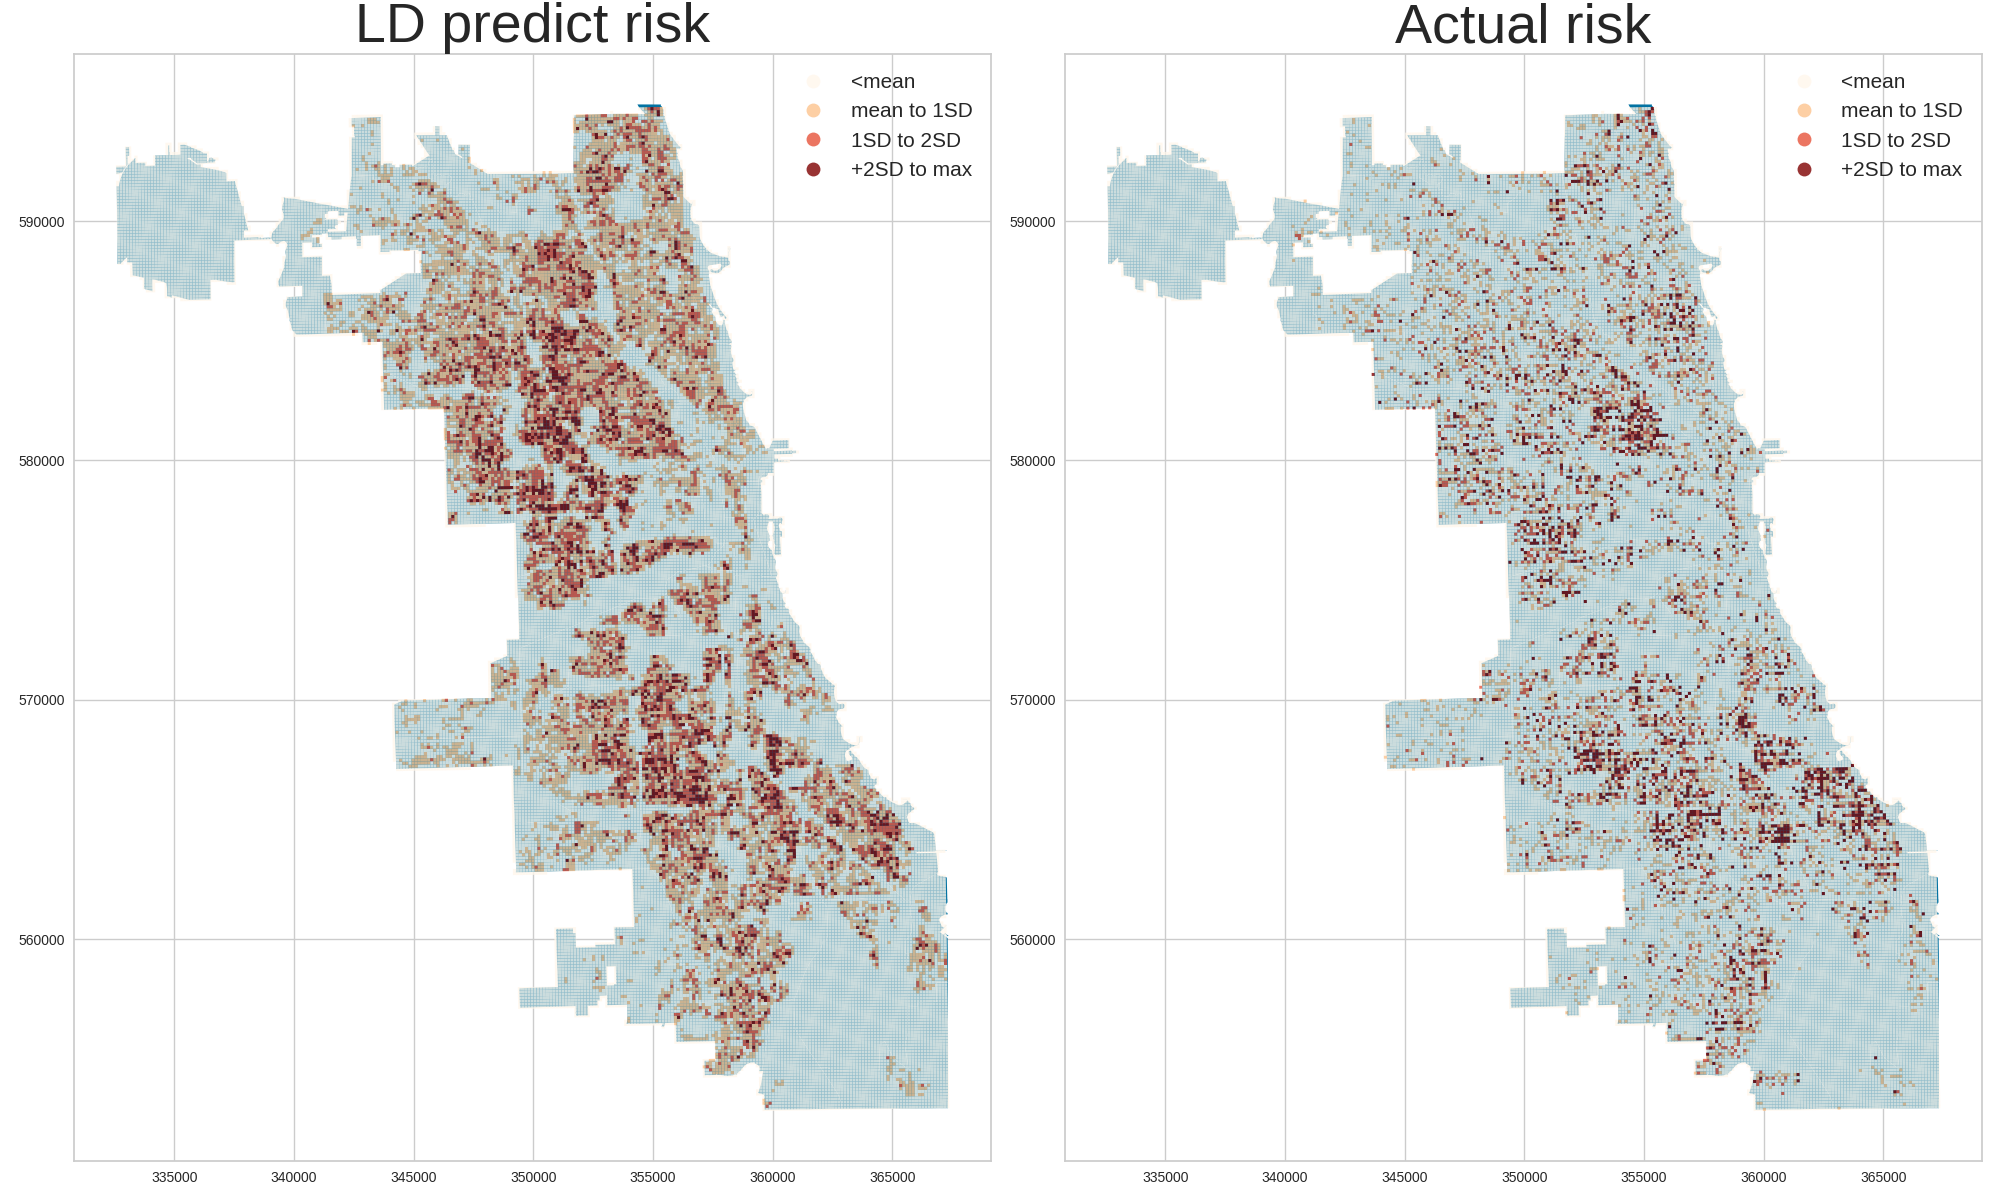
\includegraphics[scale=0.25]{./non-crime-timeseries-fig/LD_riskmap.png}
%   \caption{左:LDによるリスクマップ 右:実際のリスクマップ}
%   \label{fig:non-crime-timeseries-ld-risk}
% \end{figure}

% \begin{figure}
%   \centering % 図を中央寄せにする
%   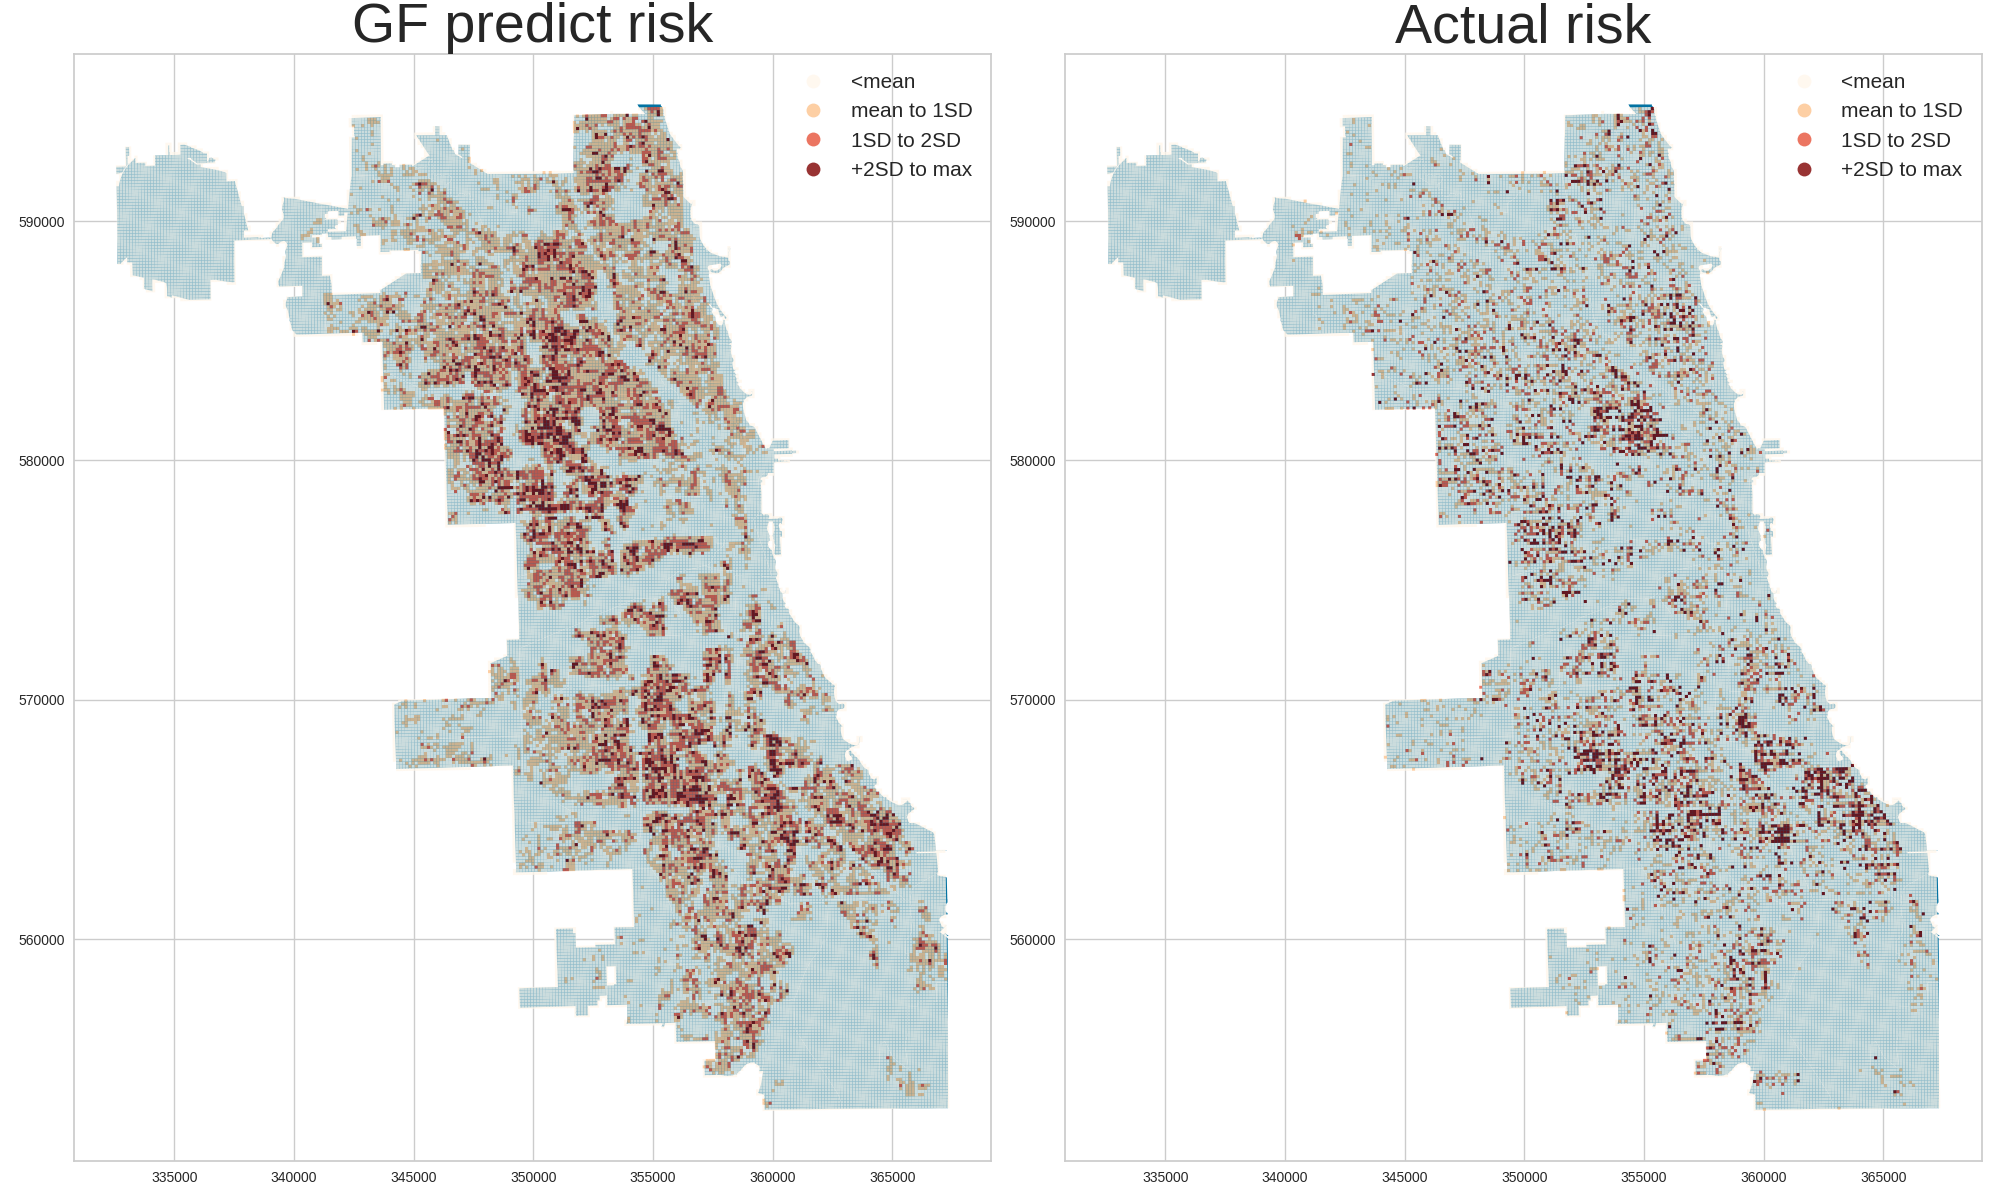
\includegraphics[scale=0.25]{./non-crime-timeseries-fig/GF_riskmap.png}
%   \caption{左:GFによるリスクマップ 右:実際のリスクマップ}
%   \label{fig:non-crime-timeseries-gf-risk}
% \end{figure}

% \begin{figure}
%   \centering % 図を中央寄せにする
%   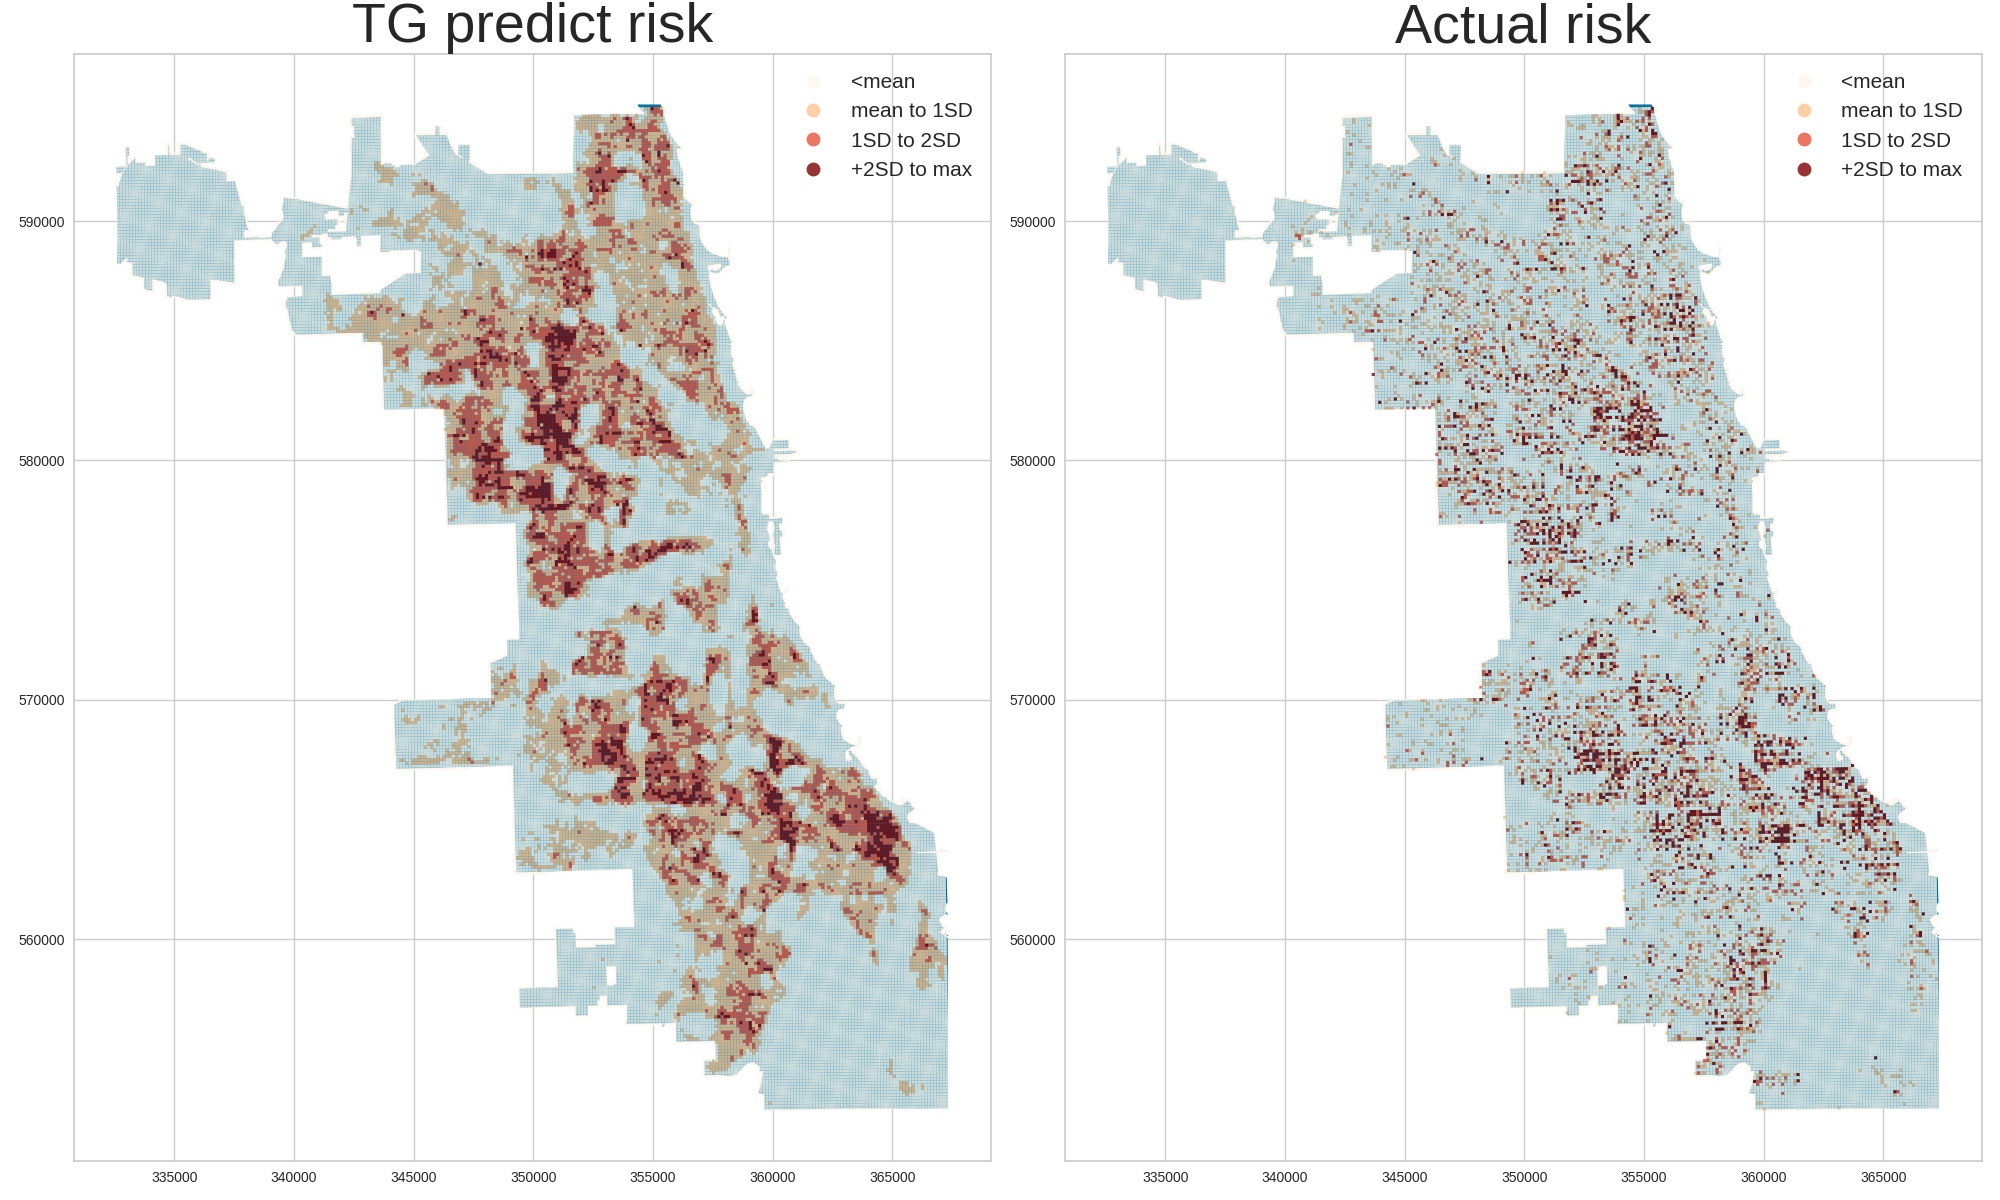
\includegraphics[scale=0.25]{./non-crime-timeseries-fig/TG_riskmap.png}
%   \caption{左:TGによるリスクマップ 右:実際のリスクマップ}
%   \label{fig:non-crime-timeseries-tg-risk}
% \end{figure}

% \begin{figure}
%   \centering % 図を中央寄せにする
%   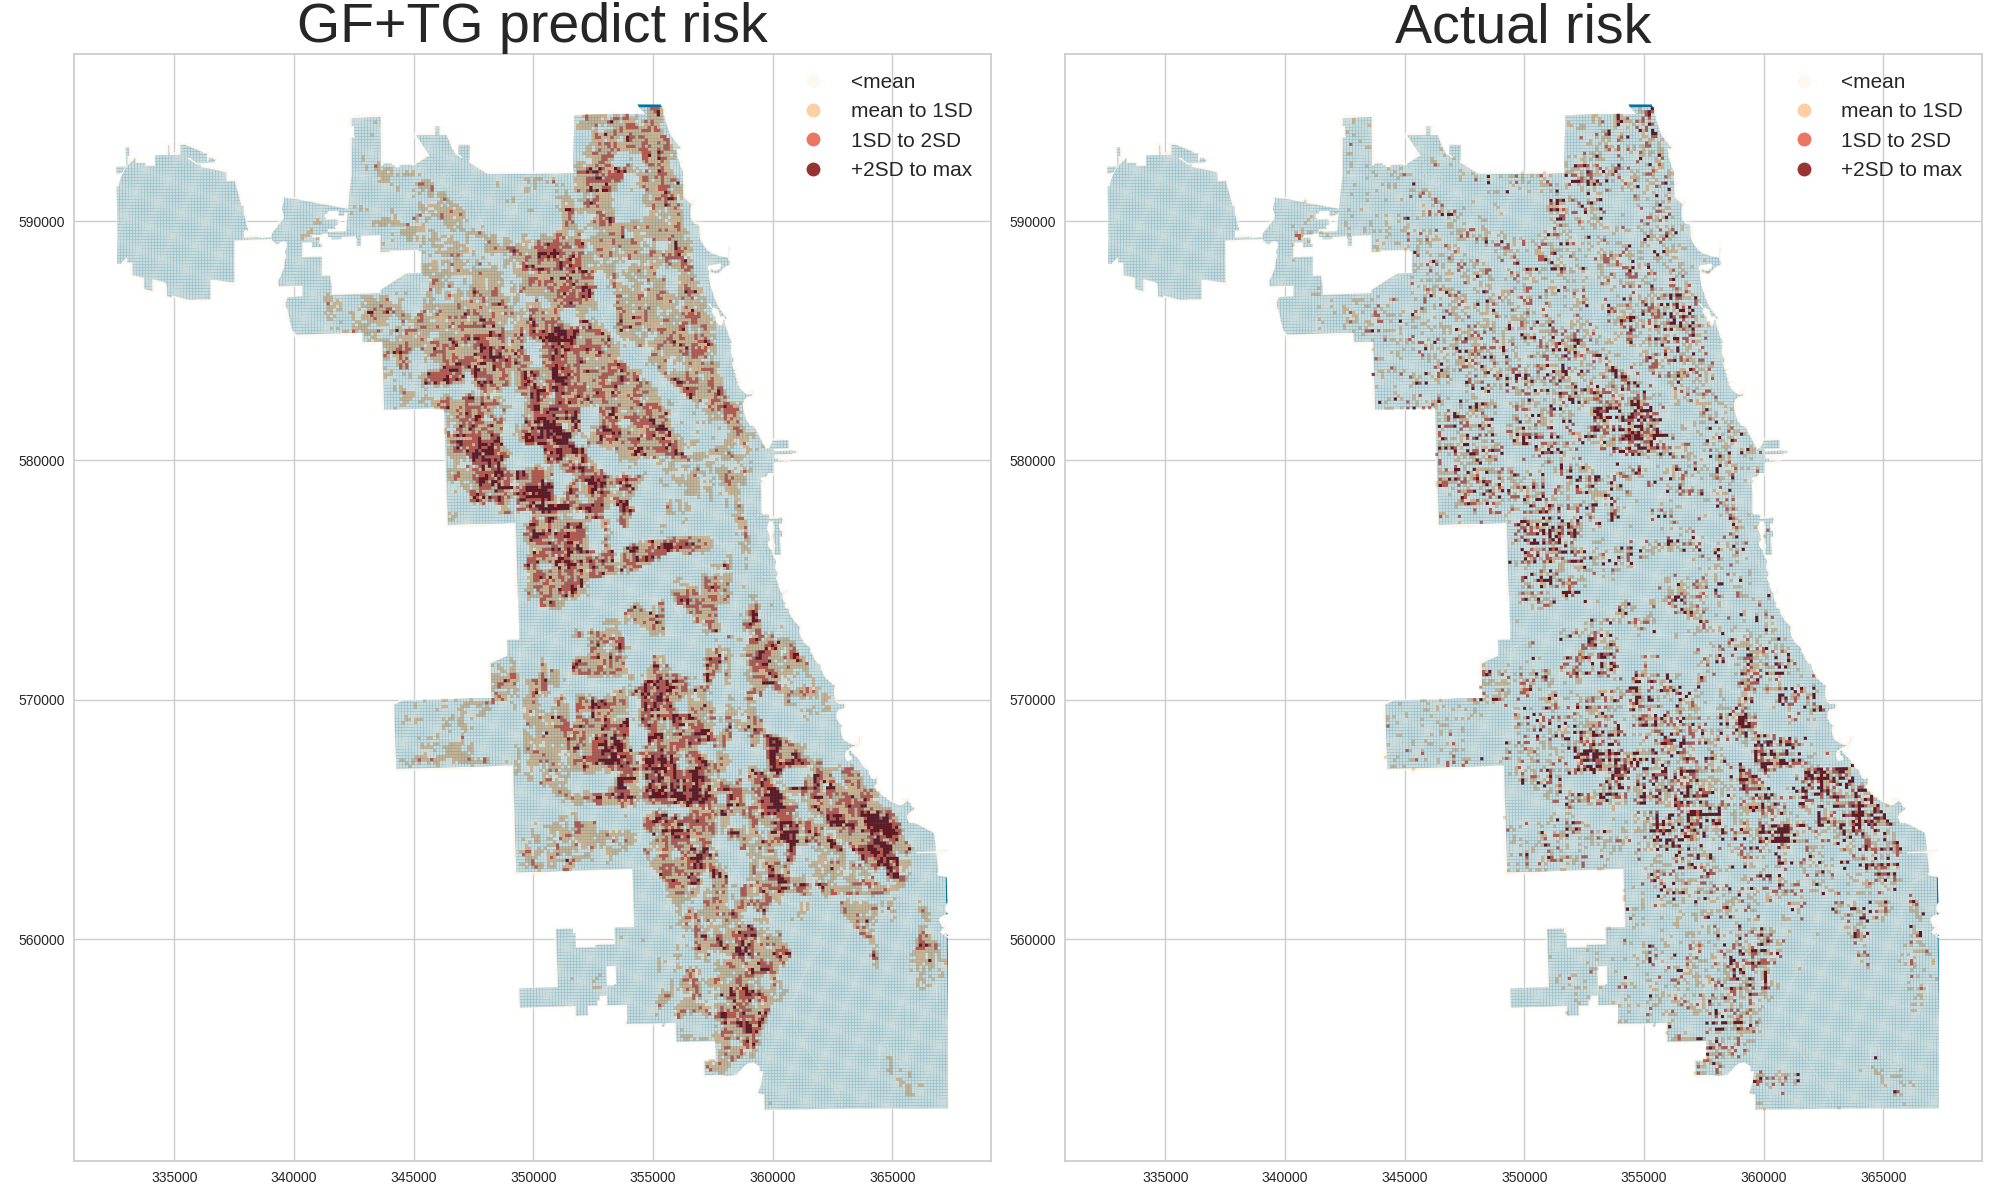
\includegraphics[scale=0.25]{./non-crime-timeseries-fig/GF+TG_riskmap.png}
%   \caption{左:FG+TGによるリスクマップ 右:実際のリスクマップ}
%   \label{fig:non-crime-timeseries-gf-tg-risk}
% \end{figure}
% %------------------------------------------
% % confusion matrix
% %------------------------------------------
% \begin{figure}
%   \centering % 図を中央寄せにする
%   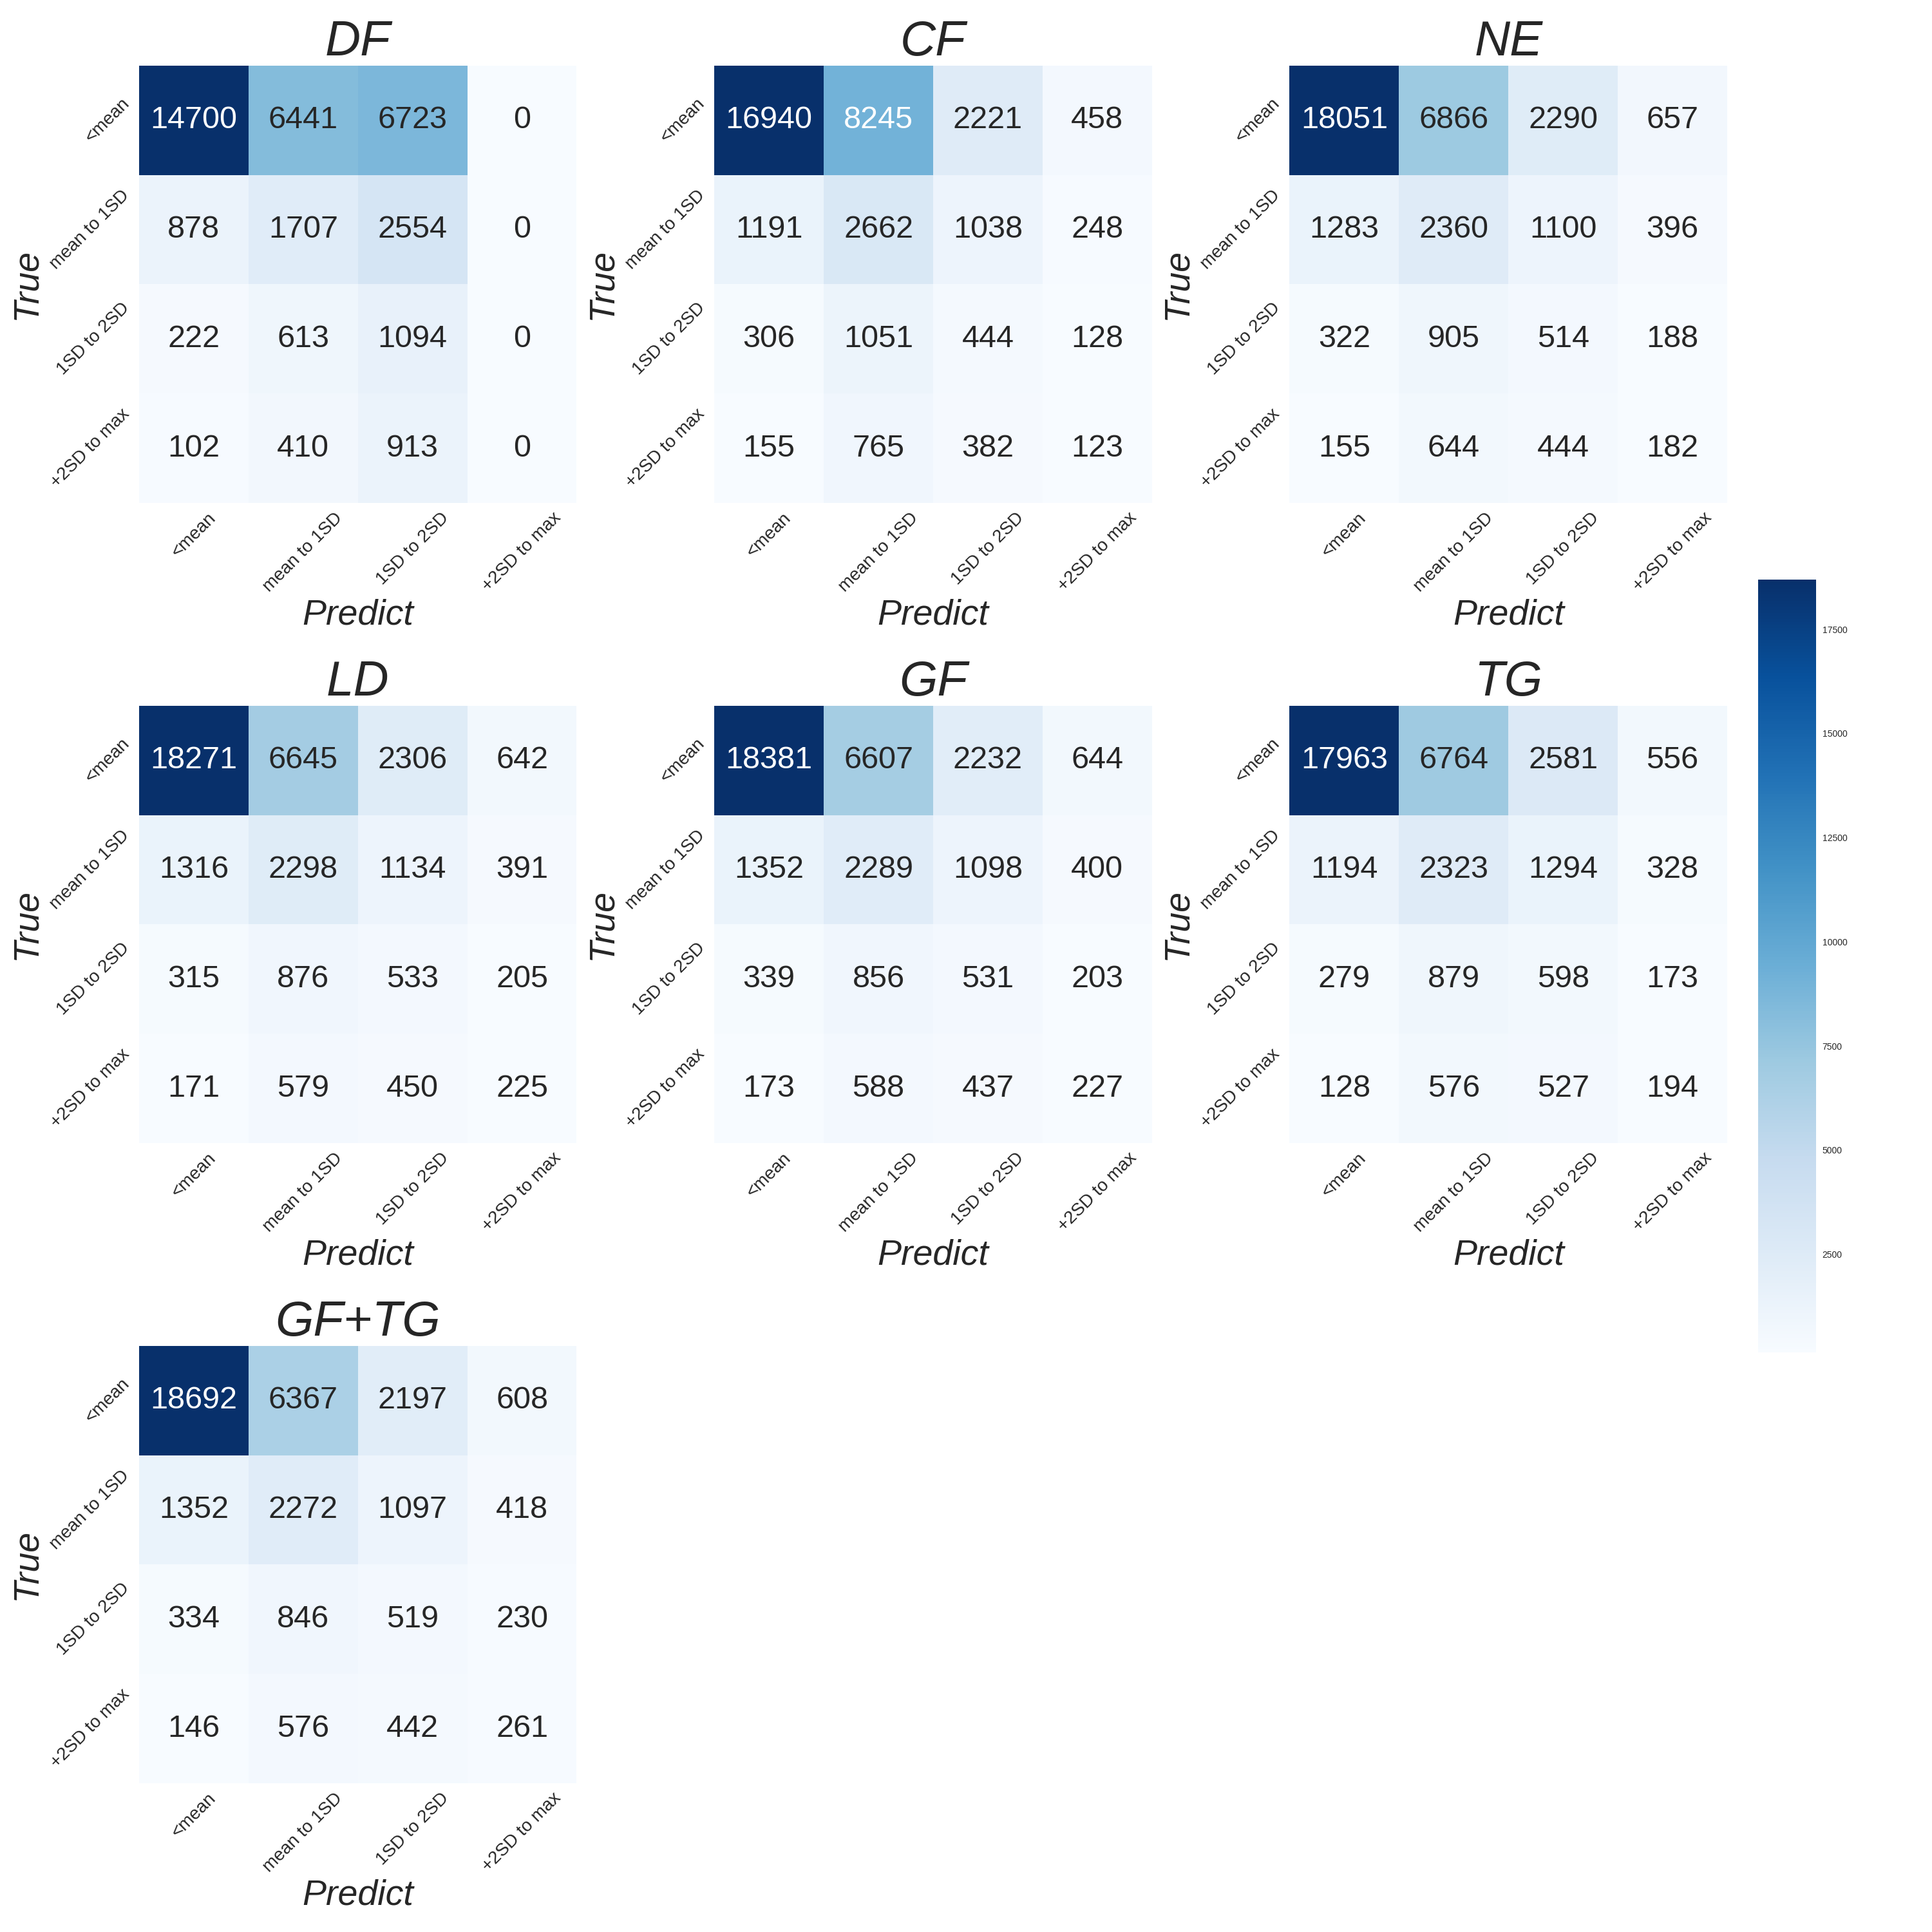
\includegraphics[scale=0.16]{./non-crime-timeseries-fig/non_crime_timeseries_four_cm.png}
%   \caption{4カテゴリーの混同行列}
%   \label{fig:non-crime-timeseries-4cm}
% \end{figure}

% \begin{figure}
%   \centering % 図を中央寄せにする
%   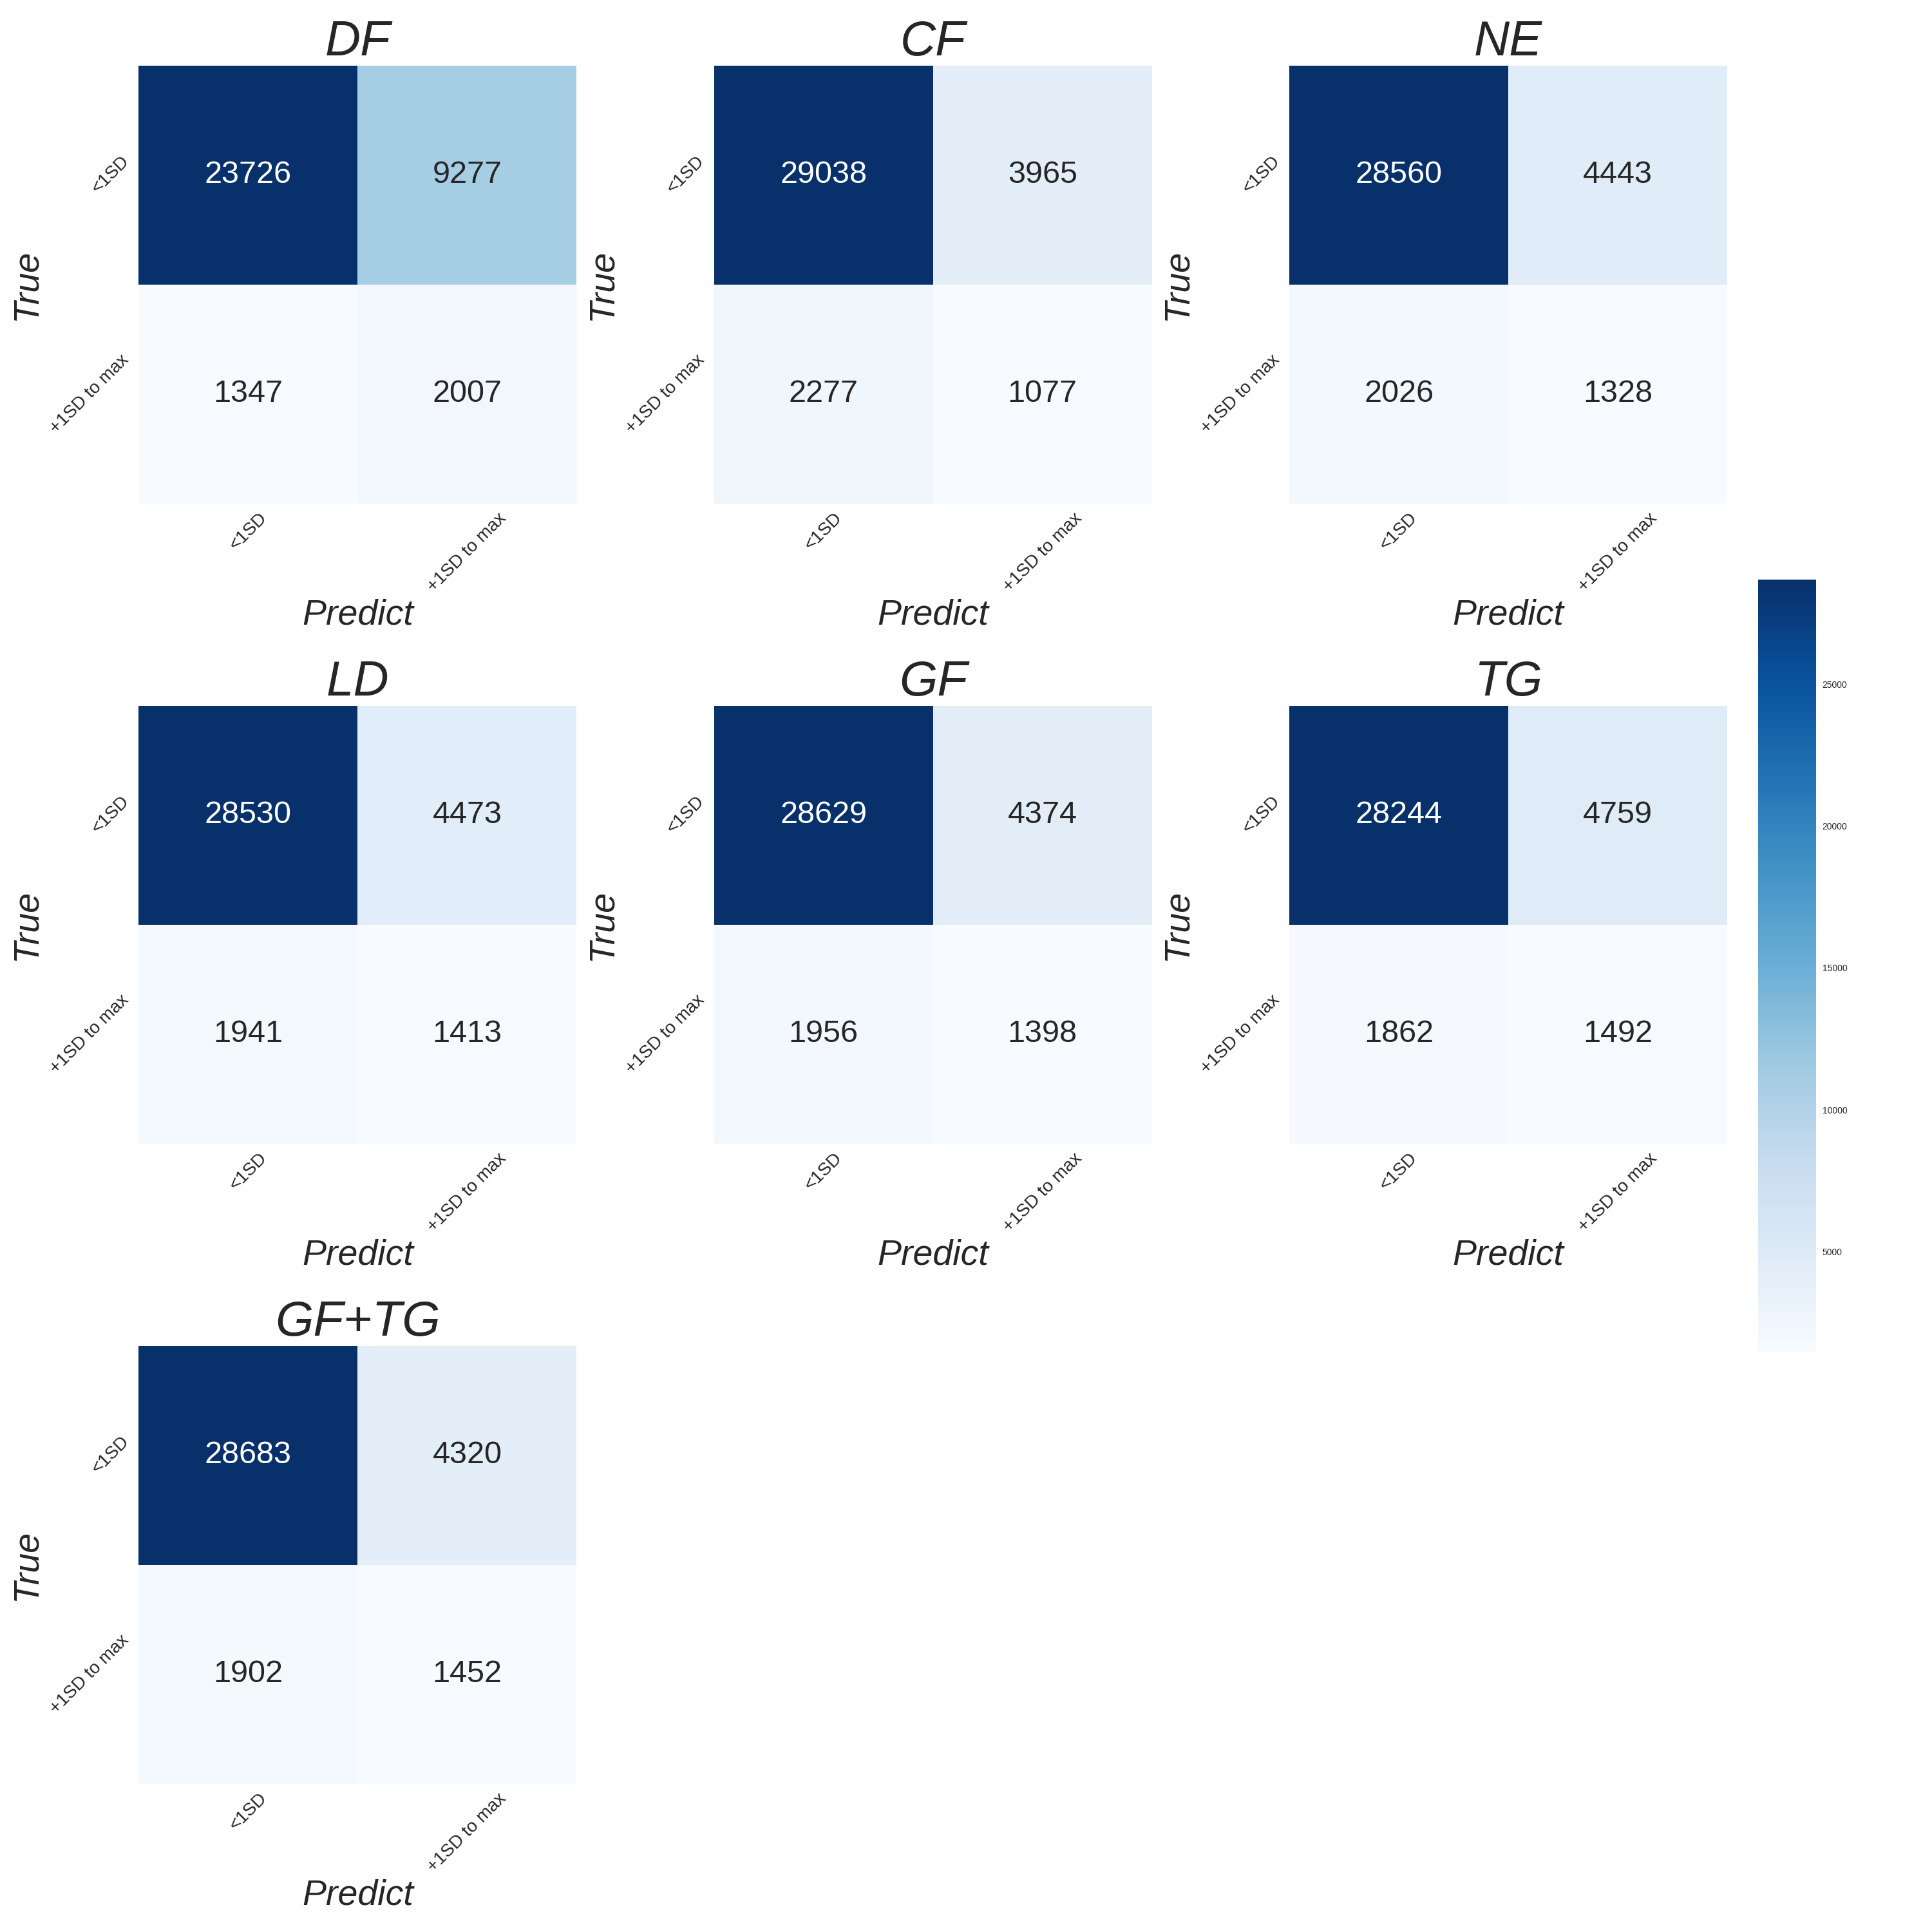
\includegraphics[scale=0.16]{./non-crime-timeseries-fig/non_crime_timeseries_two_cm.png}
%   \caption{2カテゴリーの混同行列}
%   \label{fig:non-crime-timeseries-2cm}
% \end{figure}
% ---------------------------------
% FNFPplot
% ---------------------------------
% \begin{figure}
%   \centering % 図を中央寄せにする
%   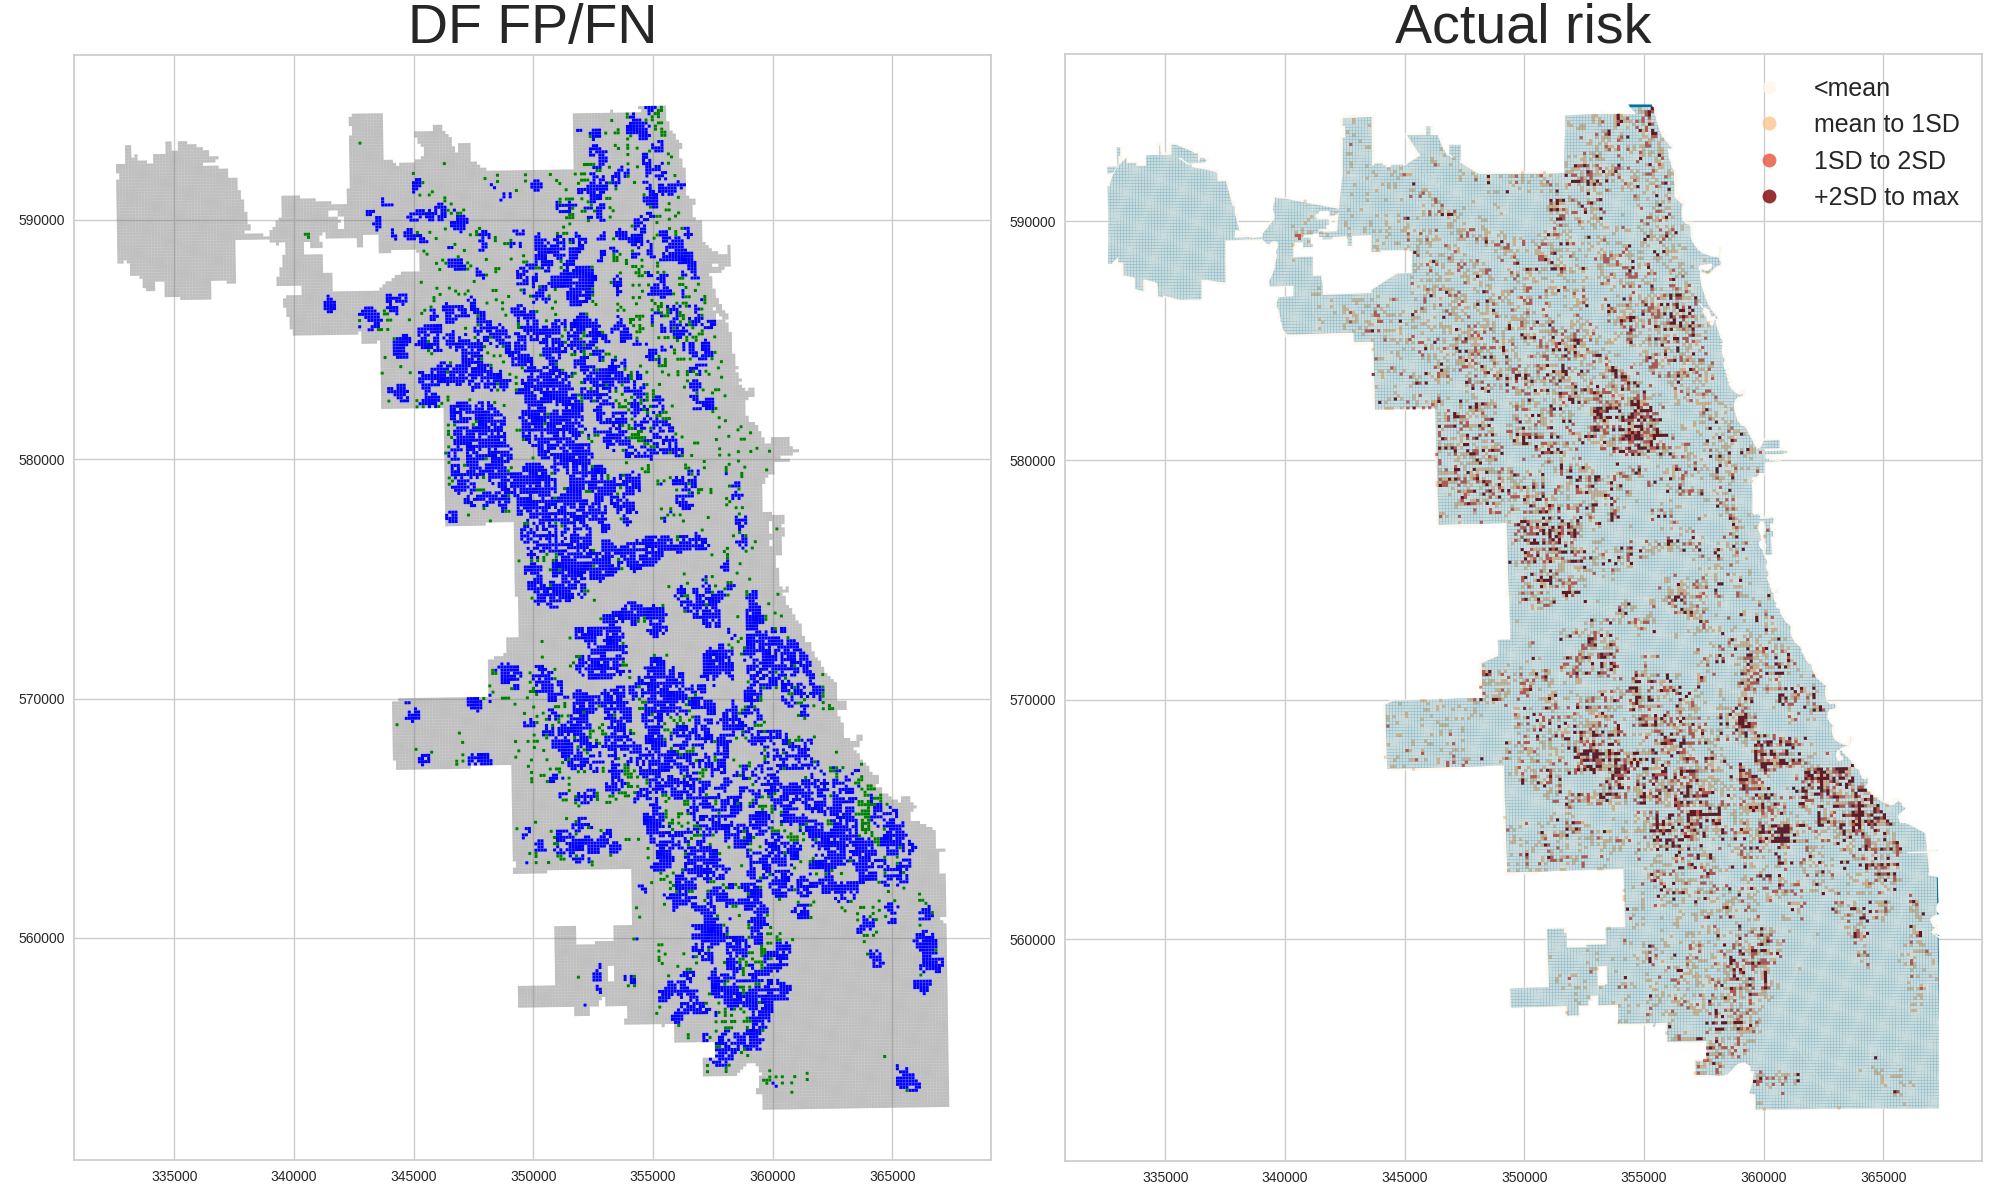
\includegraphics[scale=0.25]{./non-crime-timeseries-fig/DF_fnp.png}
%   \caption{左:DFのFPFN 右:実際のリスクマップ}
%   \label{fig:non-crime-timeseries-df-fnp}
% \end{figure}

% \begin{figure}
%   \centering % 図を中央寄せにする
%   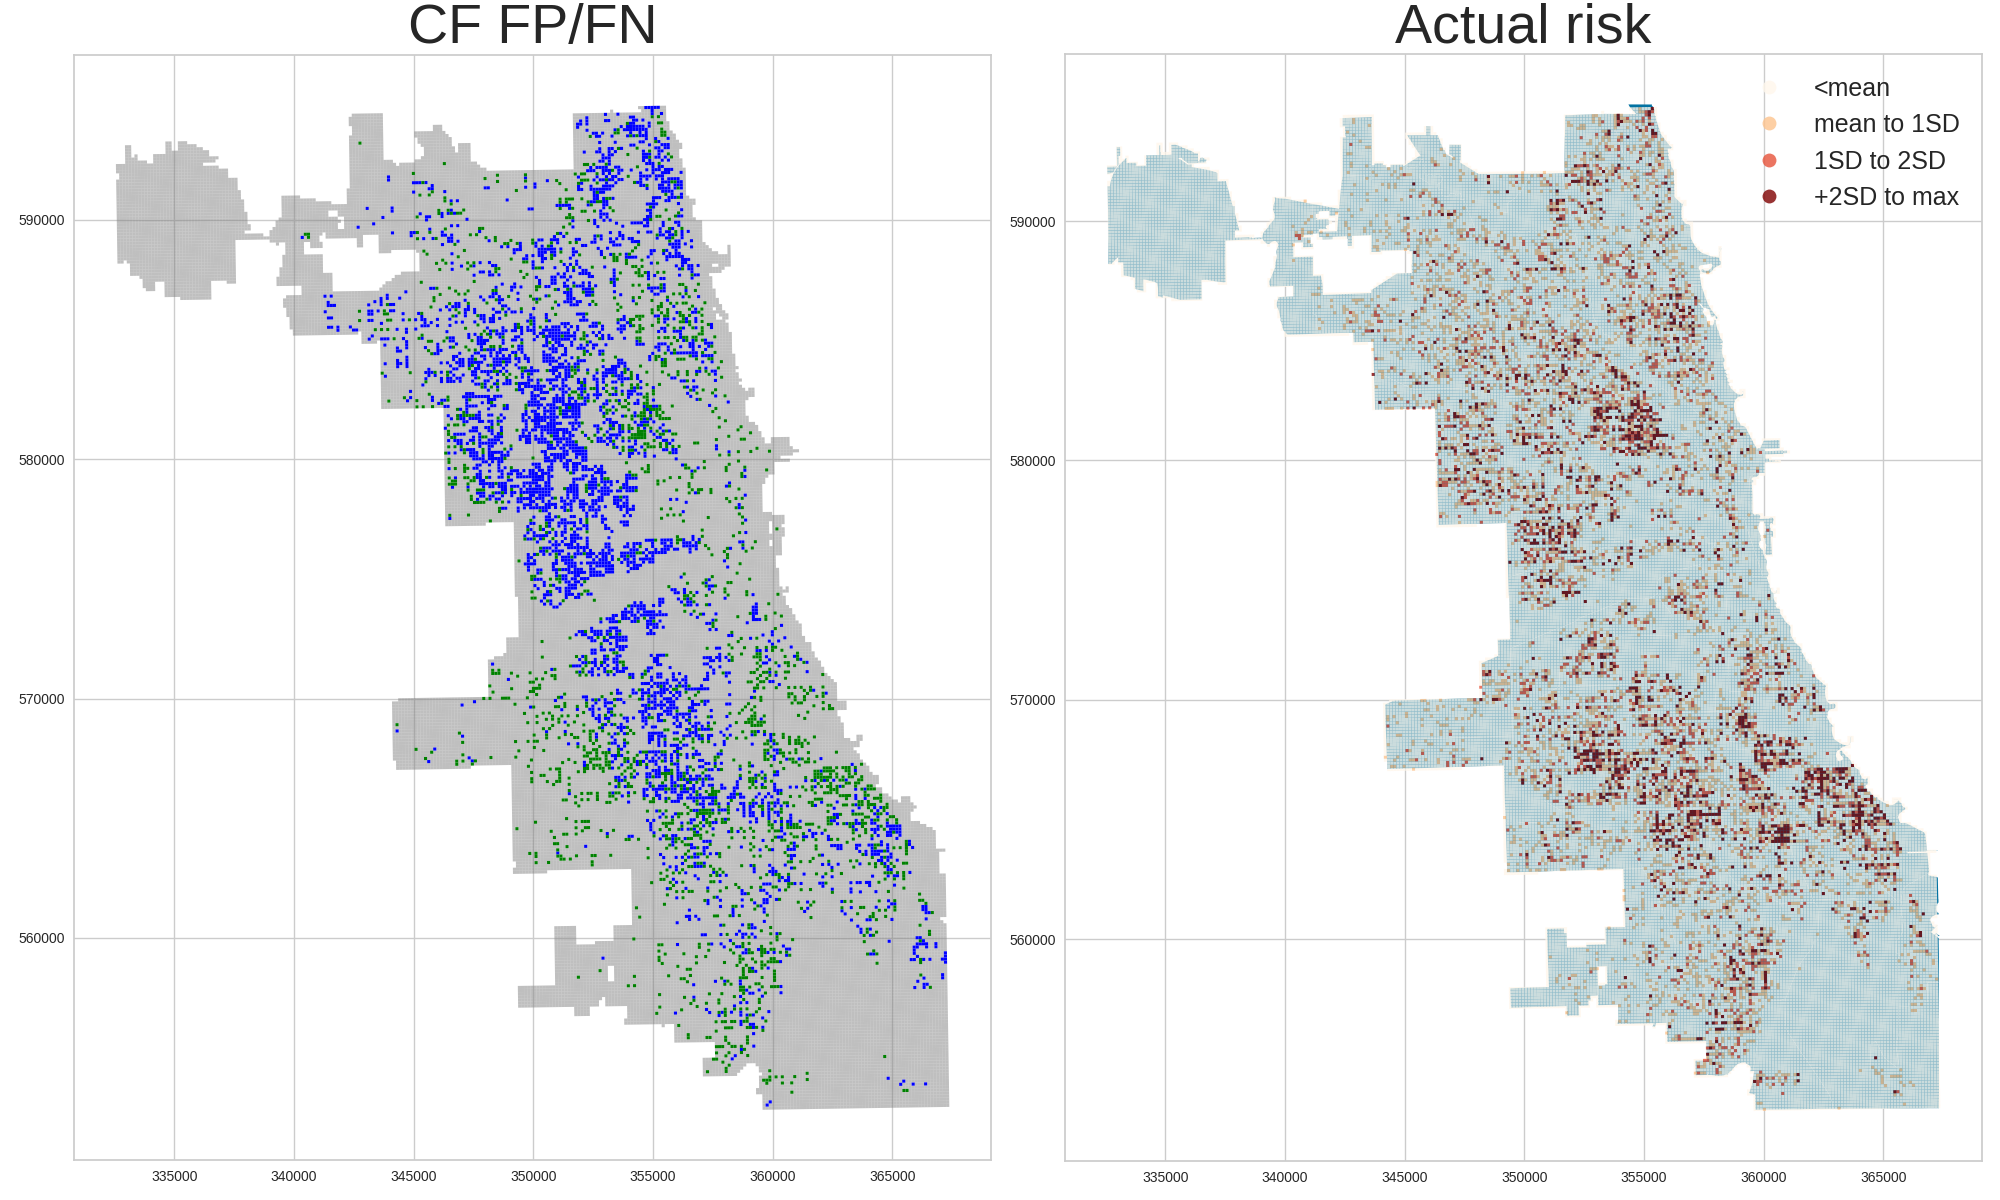
\includegraphics[scale=0.25]{./non-crime-timeseries-fig/CF_fnp.png}
%   \caption{左:CFのFPFN 右:実際のリスクマップ}
%   \label{fig:non-crime-timeseries-cf-fnp}
% \end{figure}

% \begin{figure}
%   \centering % 図を中央寄せにする
%   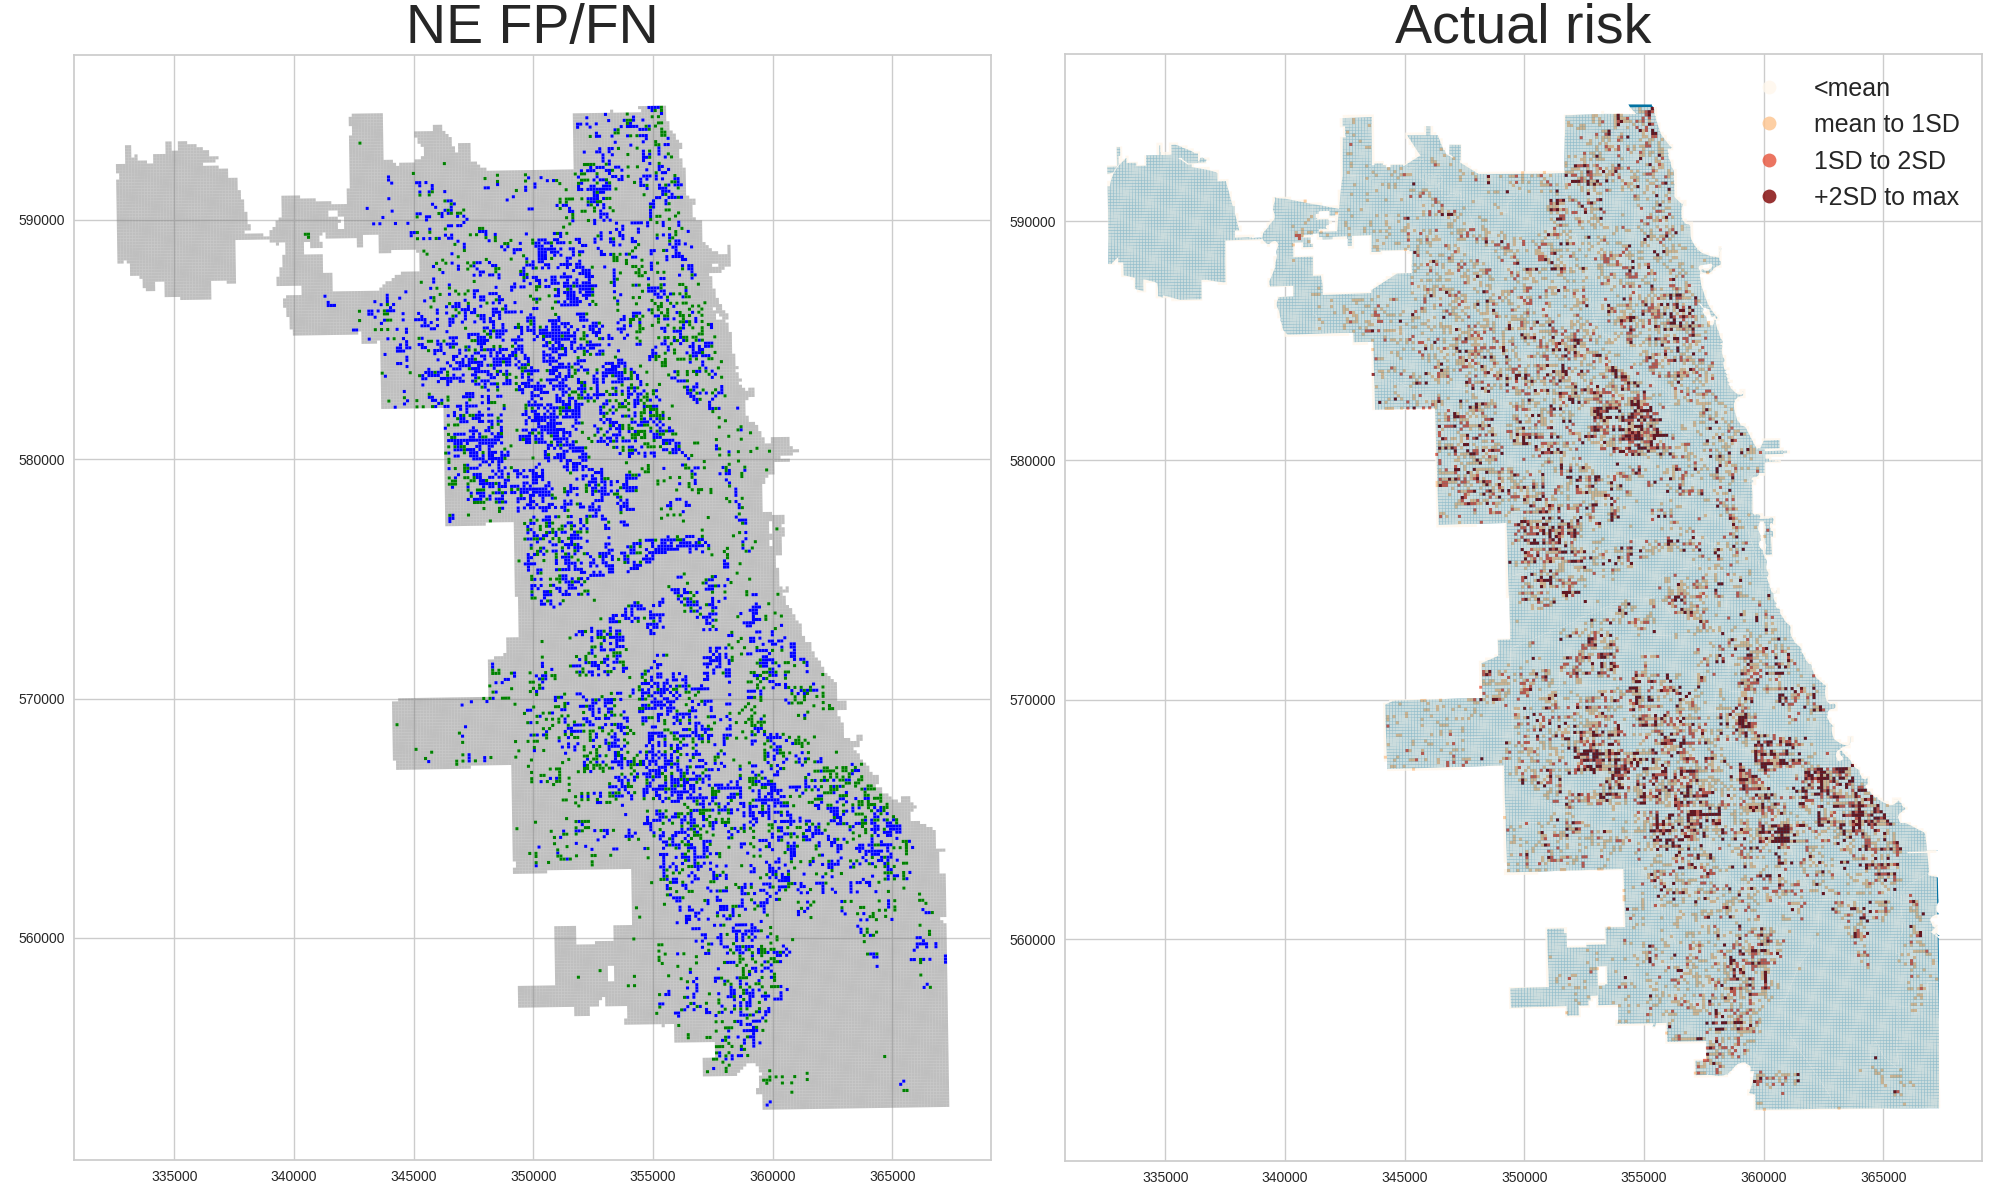
\includegraphics[scale=0.25]{./non-crime-timeseries-fig/NE_fnp.png}
%   \caption{左:NEのFPFN 右:実際のリスクマップ}
%   \label{fig:non-crime-timeseries-ne-fnp}
% \end{figure}

% \begin{figure}
%   \centering % 図を中央寄せにする
%   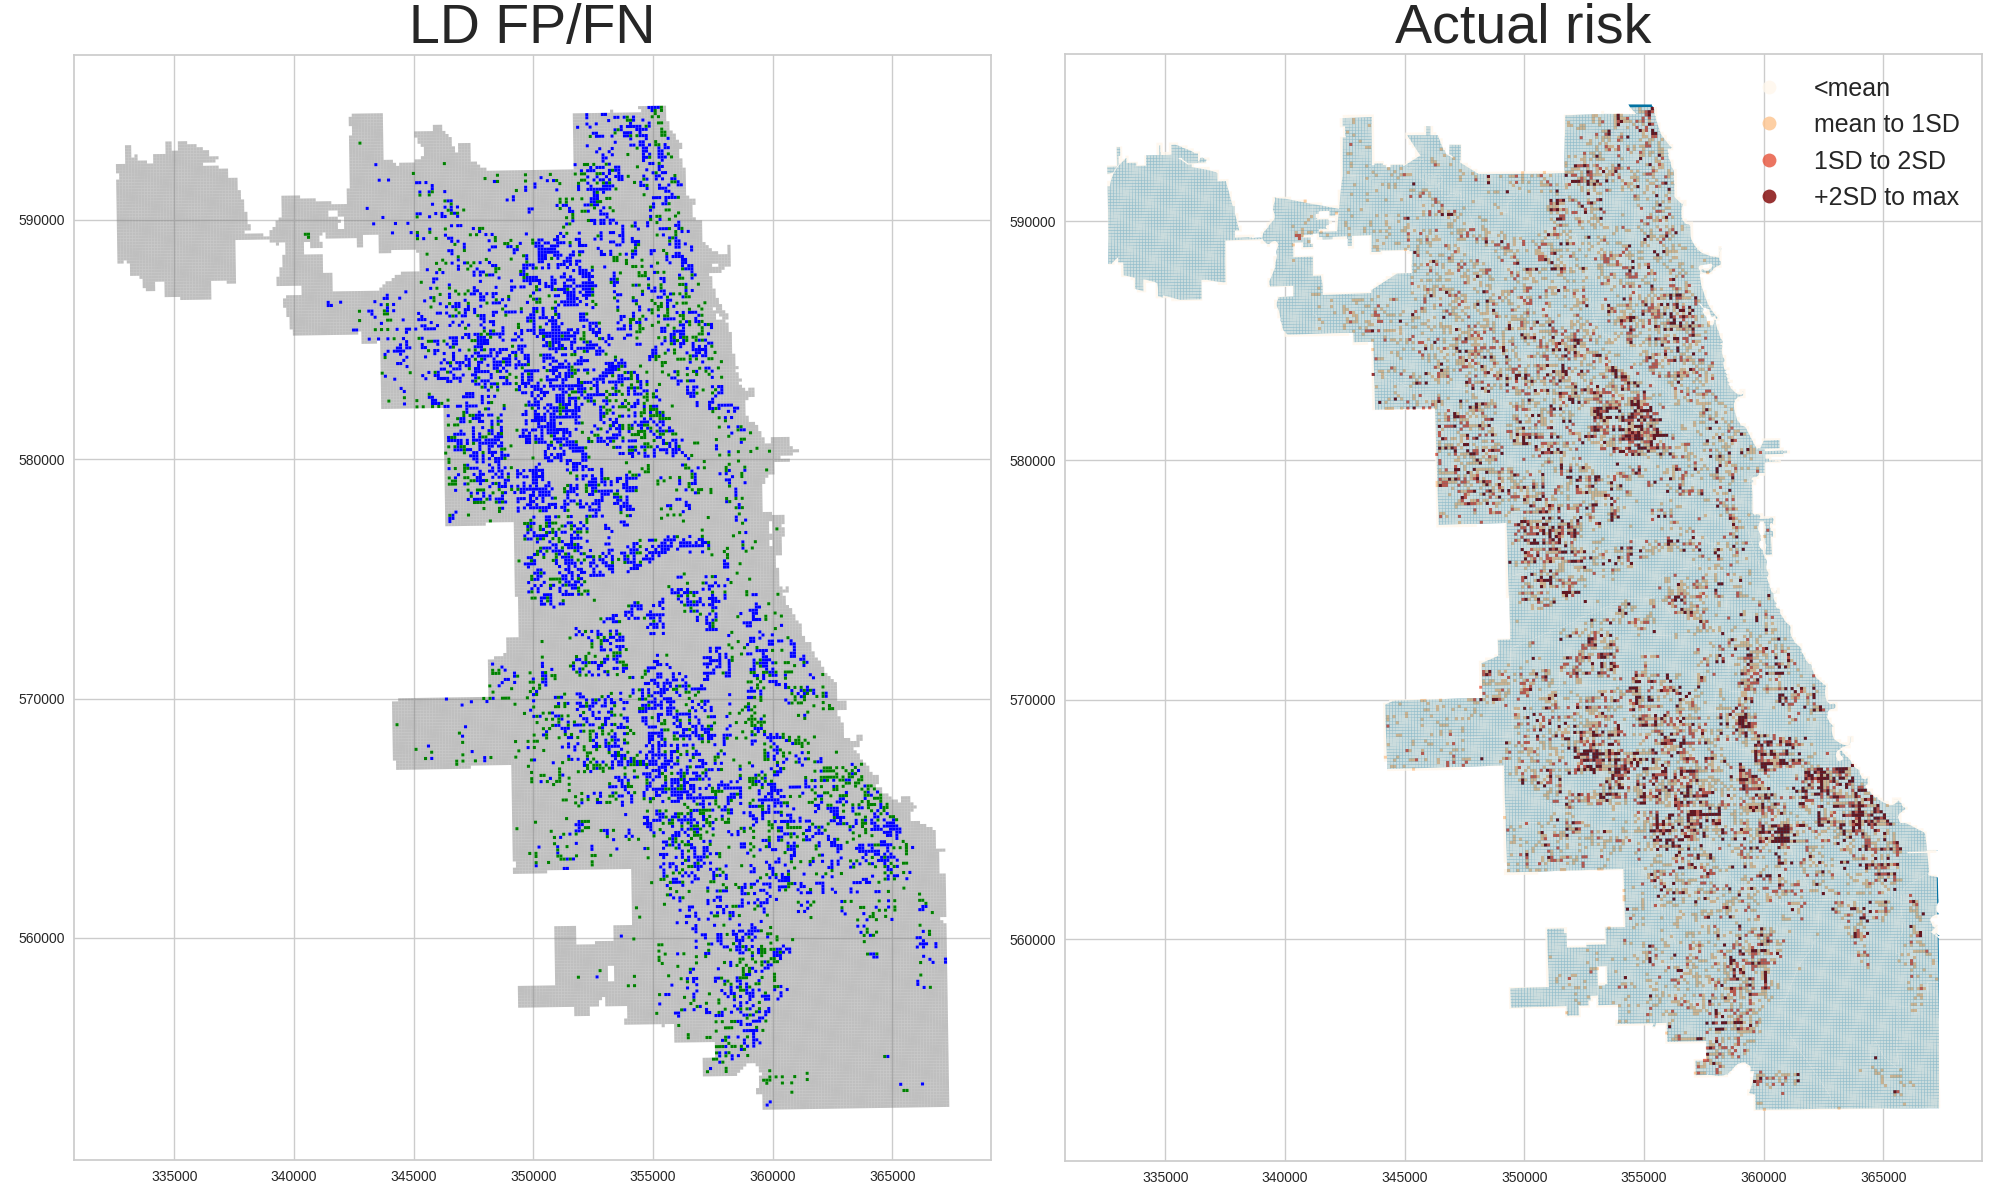
\includegraphics[scale=0.25]{./non-crime-timeseries-fig/LD_fnp.png}
%   \caption{左:LDのFPFN 右:実際のリスクマップ}
%   \label{fig:non-crime-timeseries-ld-fnp}
% \end{figure}

% \begin{figure}
%   \centering % 図を中央寄せにする
%   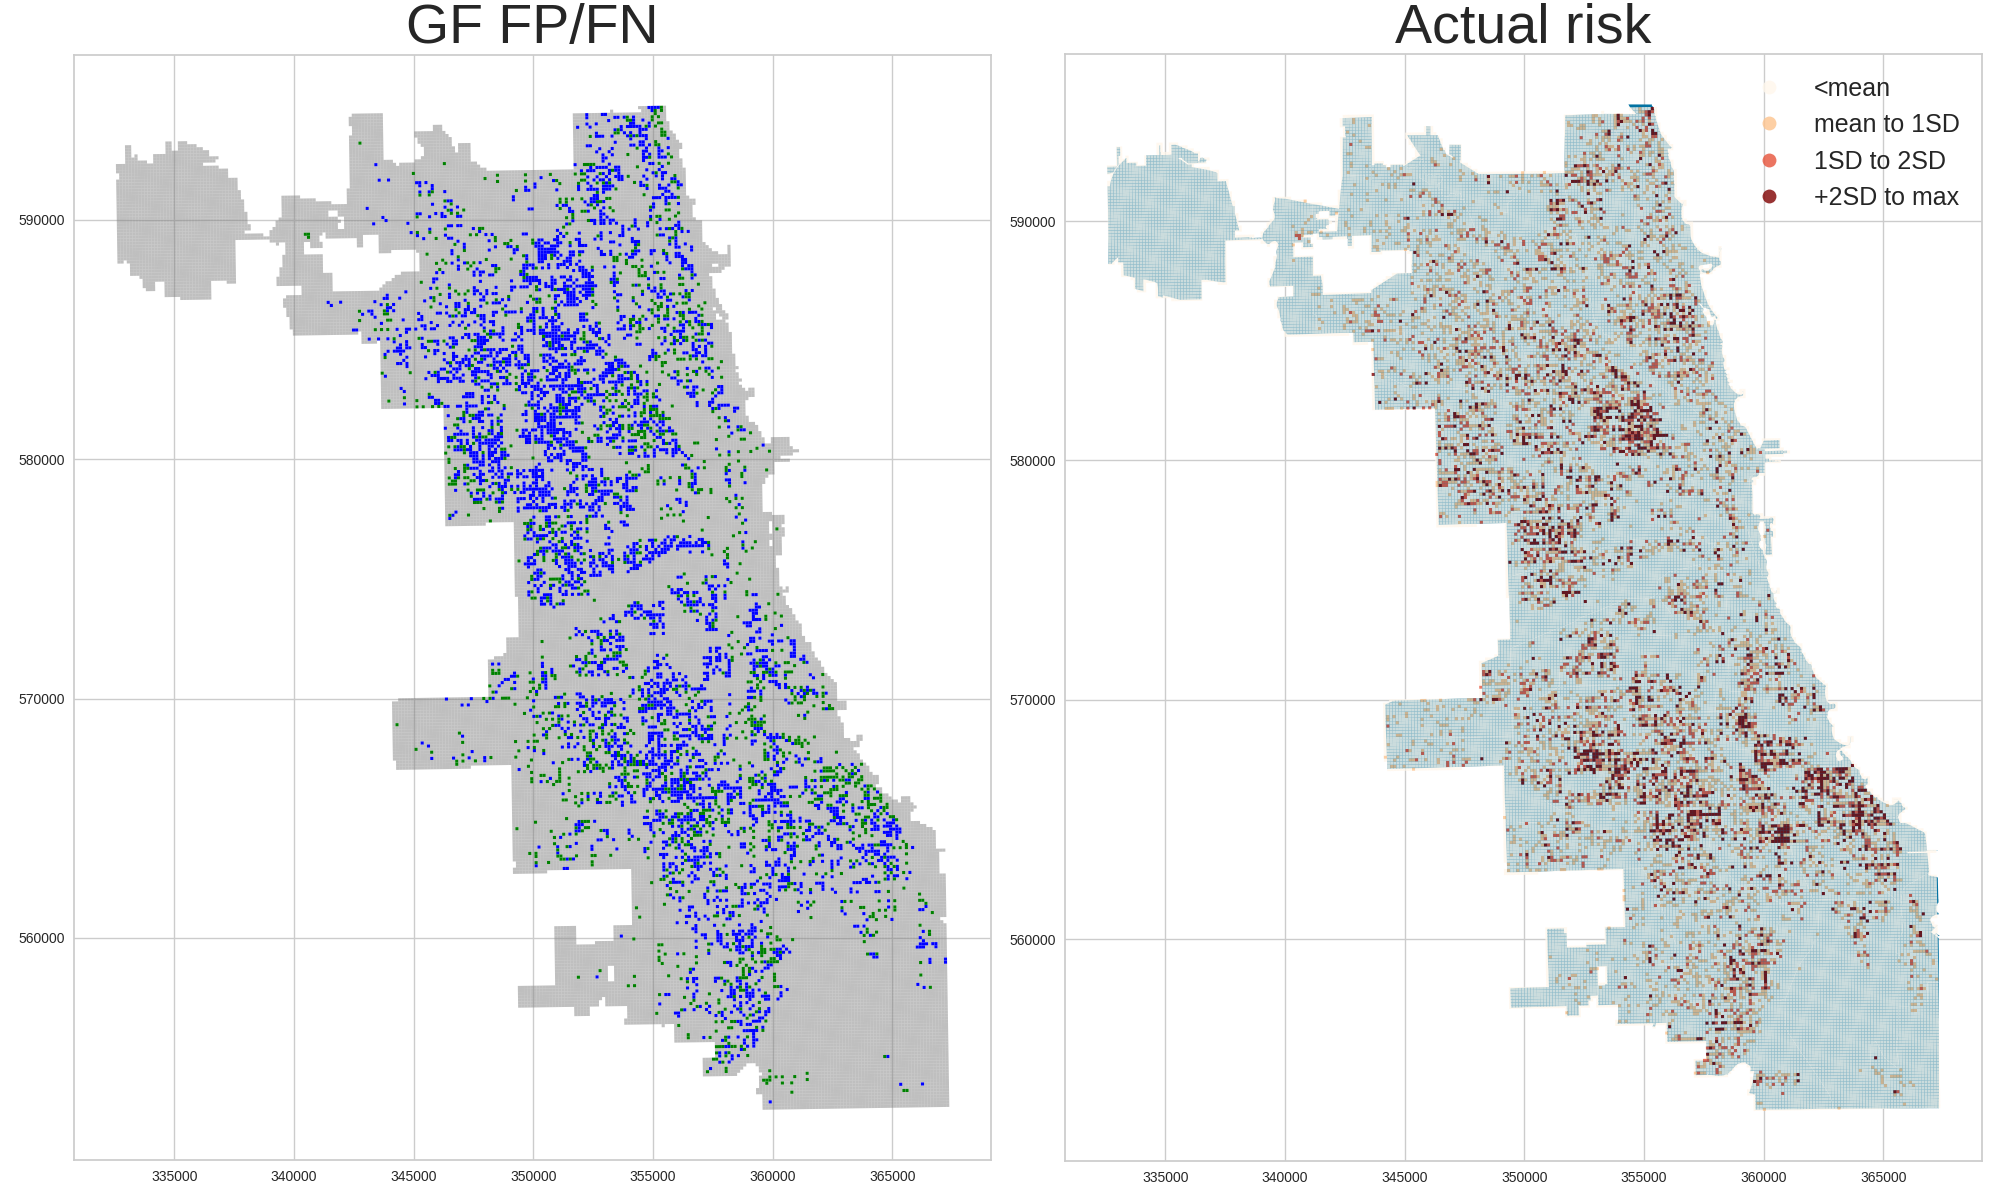
\includegraphics[scale=0.25]{./non-crime-timeseries-fig/GF_fnp.png}
%   \caption{左:GFのFPFN 右:実際のリスクマップ}
%   \label{fig:non-crime-timeseries-gf-fnp}
% \end{figure}

% \begin{figure}
%   \centering % 図を中央寄せにする
%   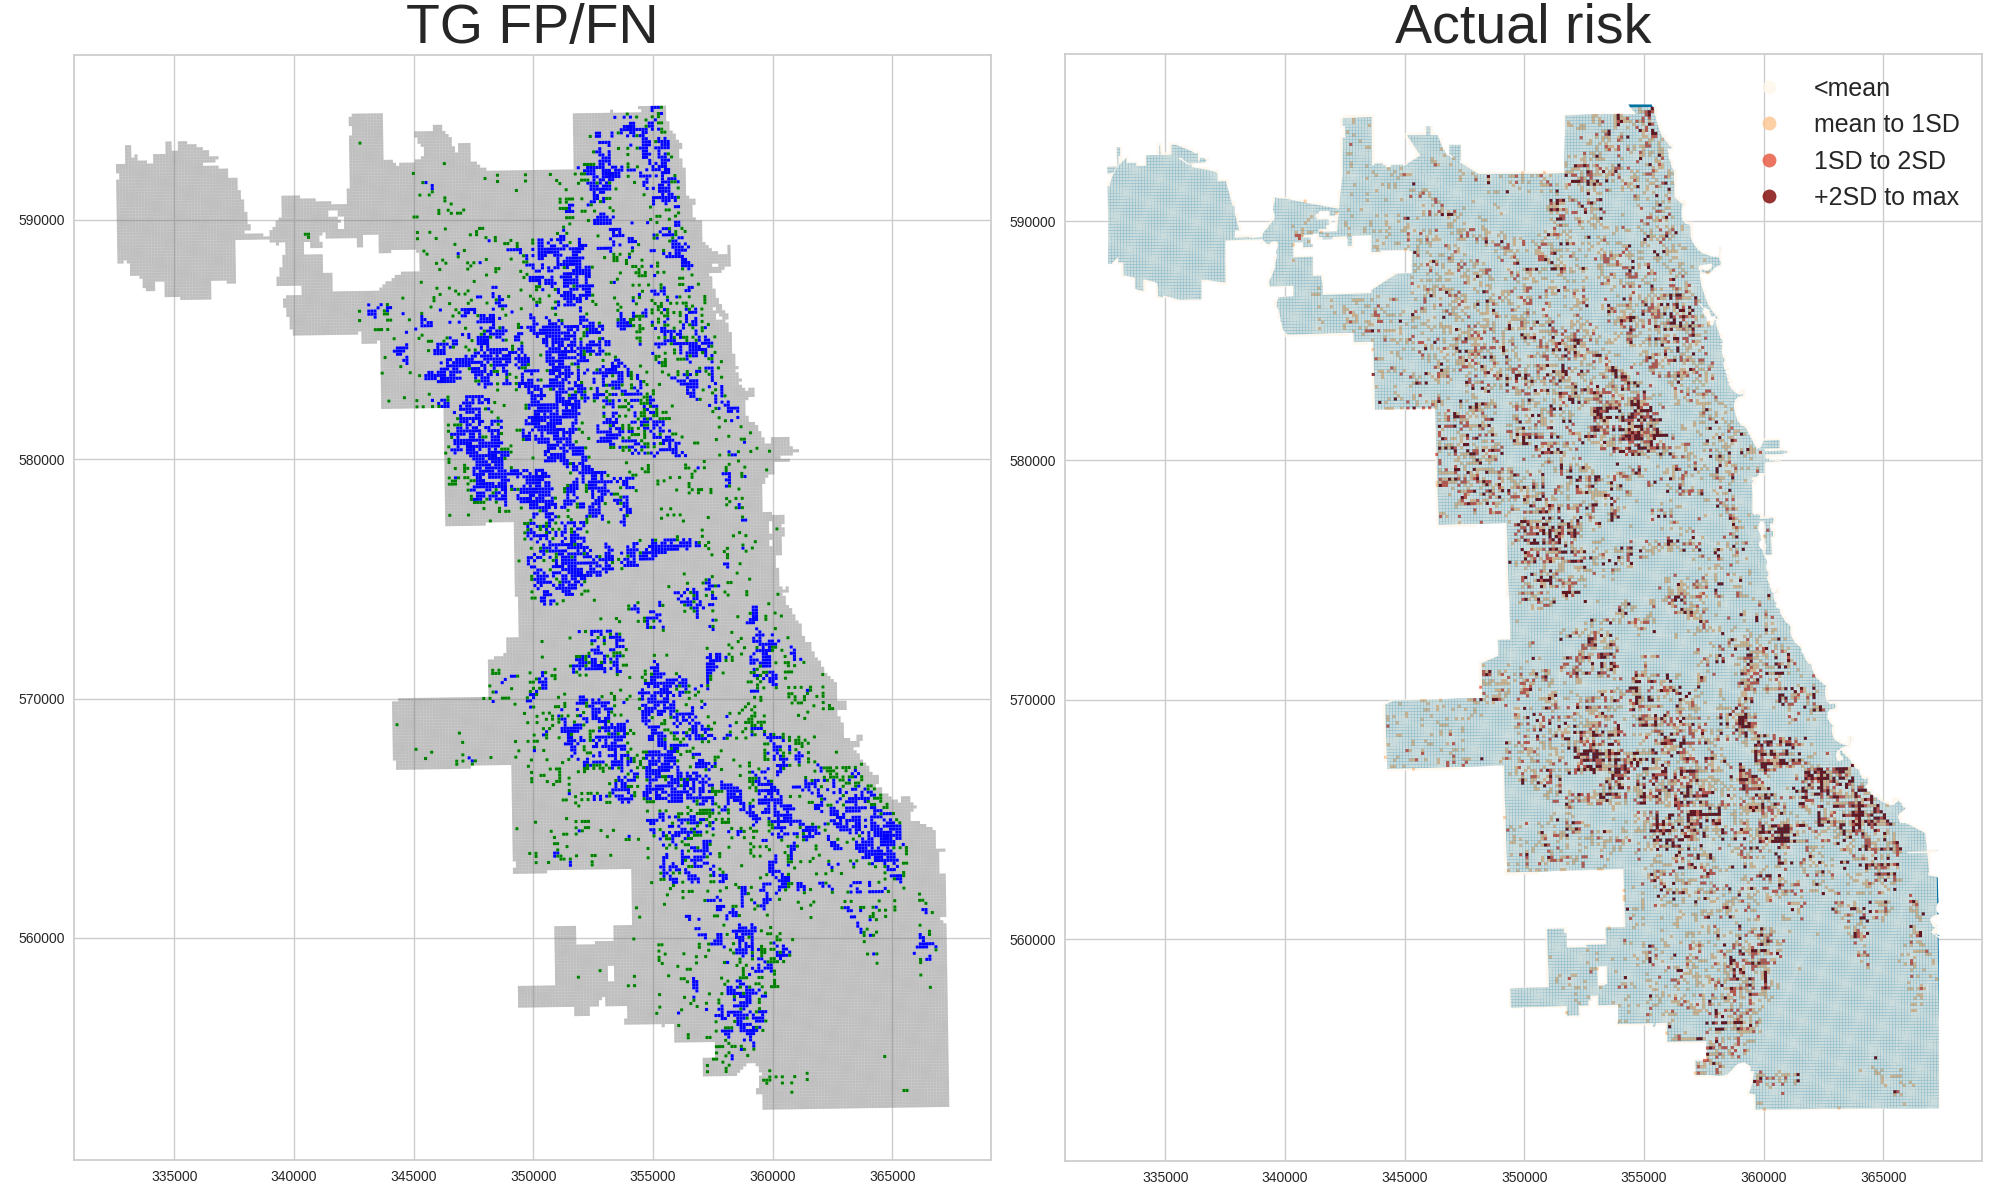
\includegraphics[scale=0.25]{./non-crime-timeseries-fig/TG_fnp.png}
%   \caption{左:TGのFPFN 右:実際のリスクマップ}
%   \label{fig:non-crime-timeseries-tg-fnp}
% \end{figure}

% \begin{figure}
%   \centering % 図を中央寄せにする
%   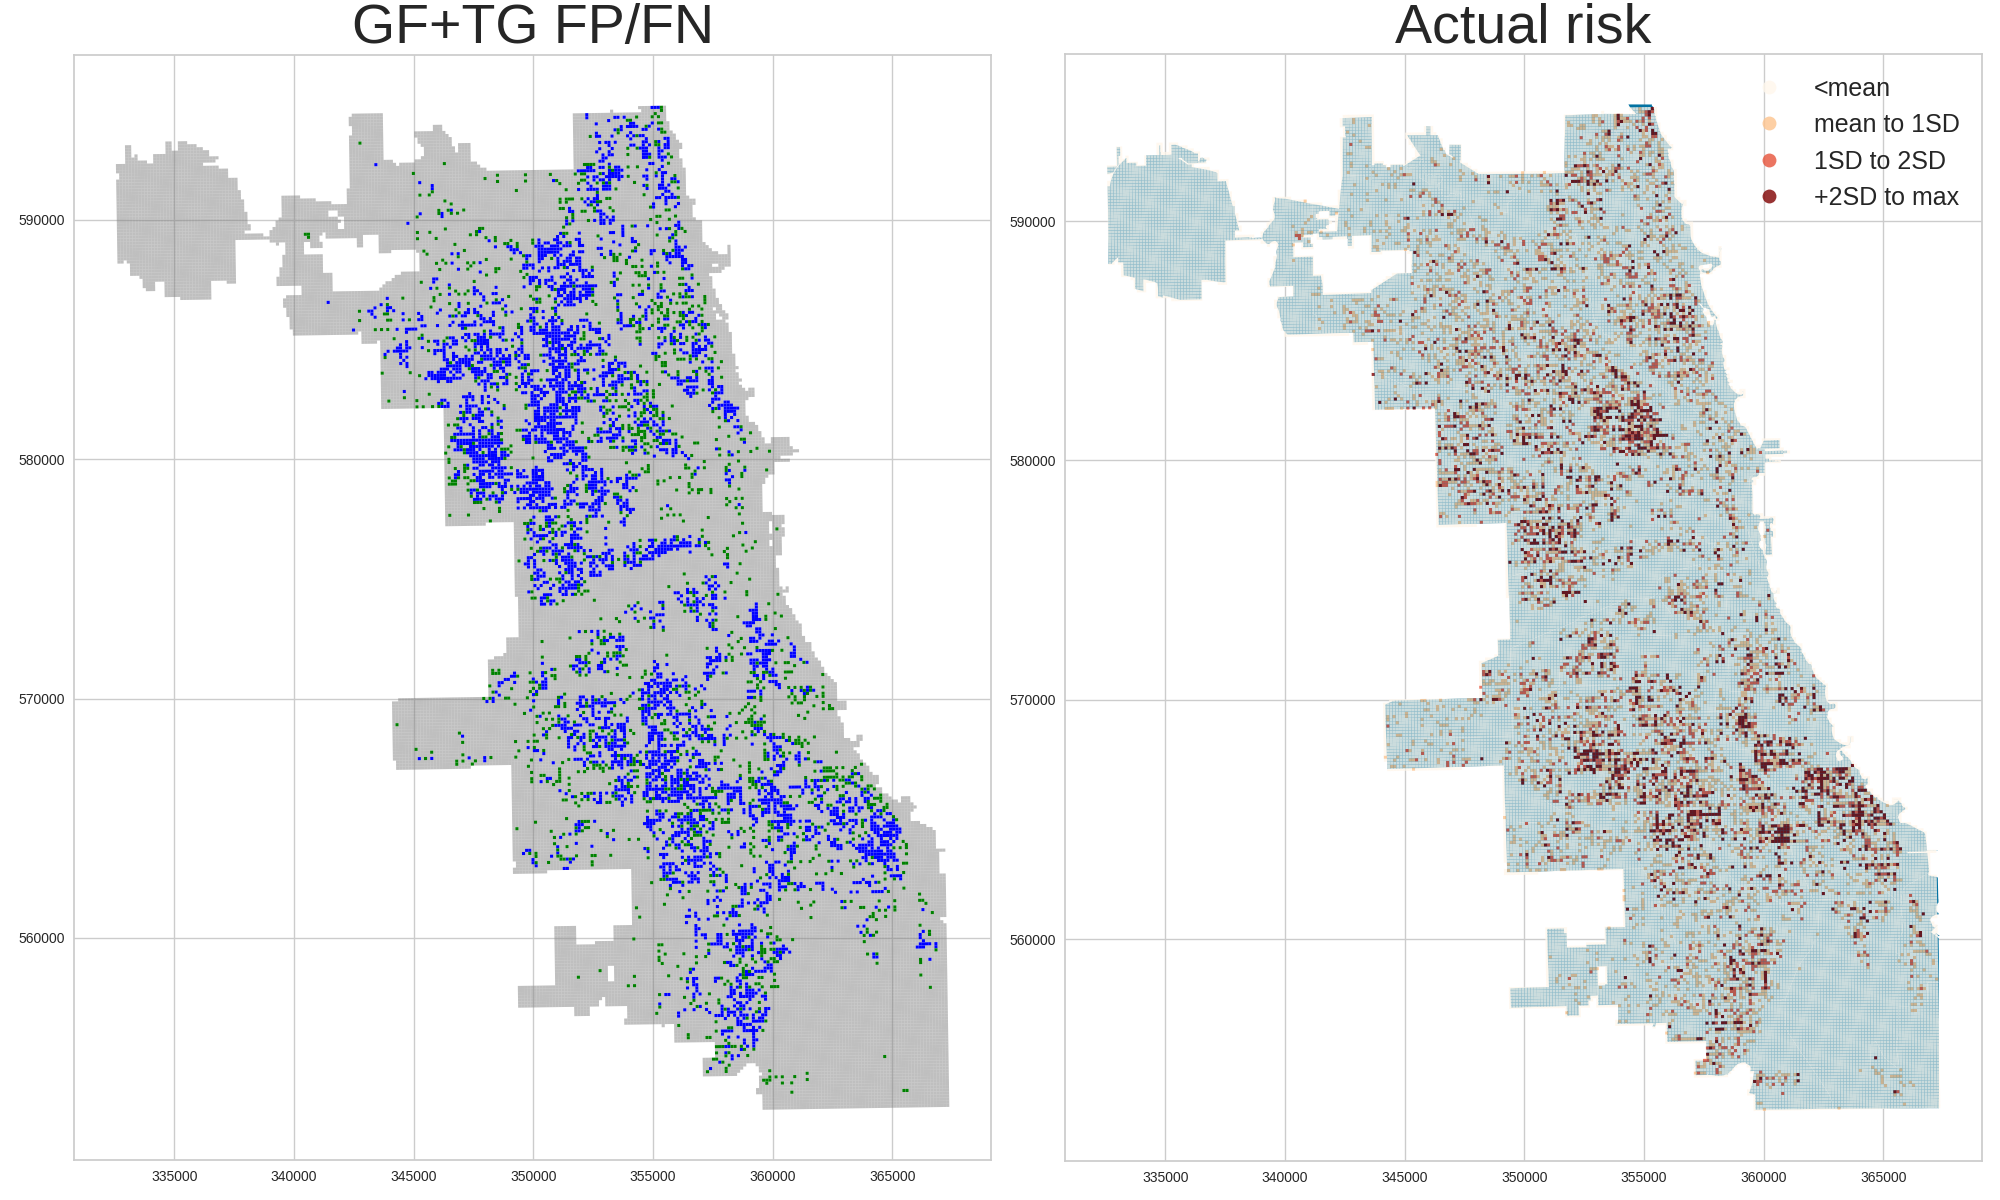
\includegraphics[scale=0.25]{./non-crime-timeseries-fig/GF+TG_fnp.png}
%   \caption{左:GF+TGのFPFN 右:実際のリスクマップ}
%   \label{fig:non-crime-timeseries-gf-tg-fnp}
% \end{figure}
% %------------------------------------------
% % ROC curve
% %------------------------------------------
% また,各モデルのROC曲線を図\ref{fig:non-crime-timeseries-roc}に示した.

% \begin{figure}
%   \centering % 図を中央寄せにする
%   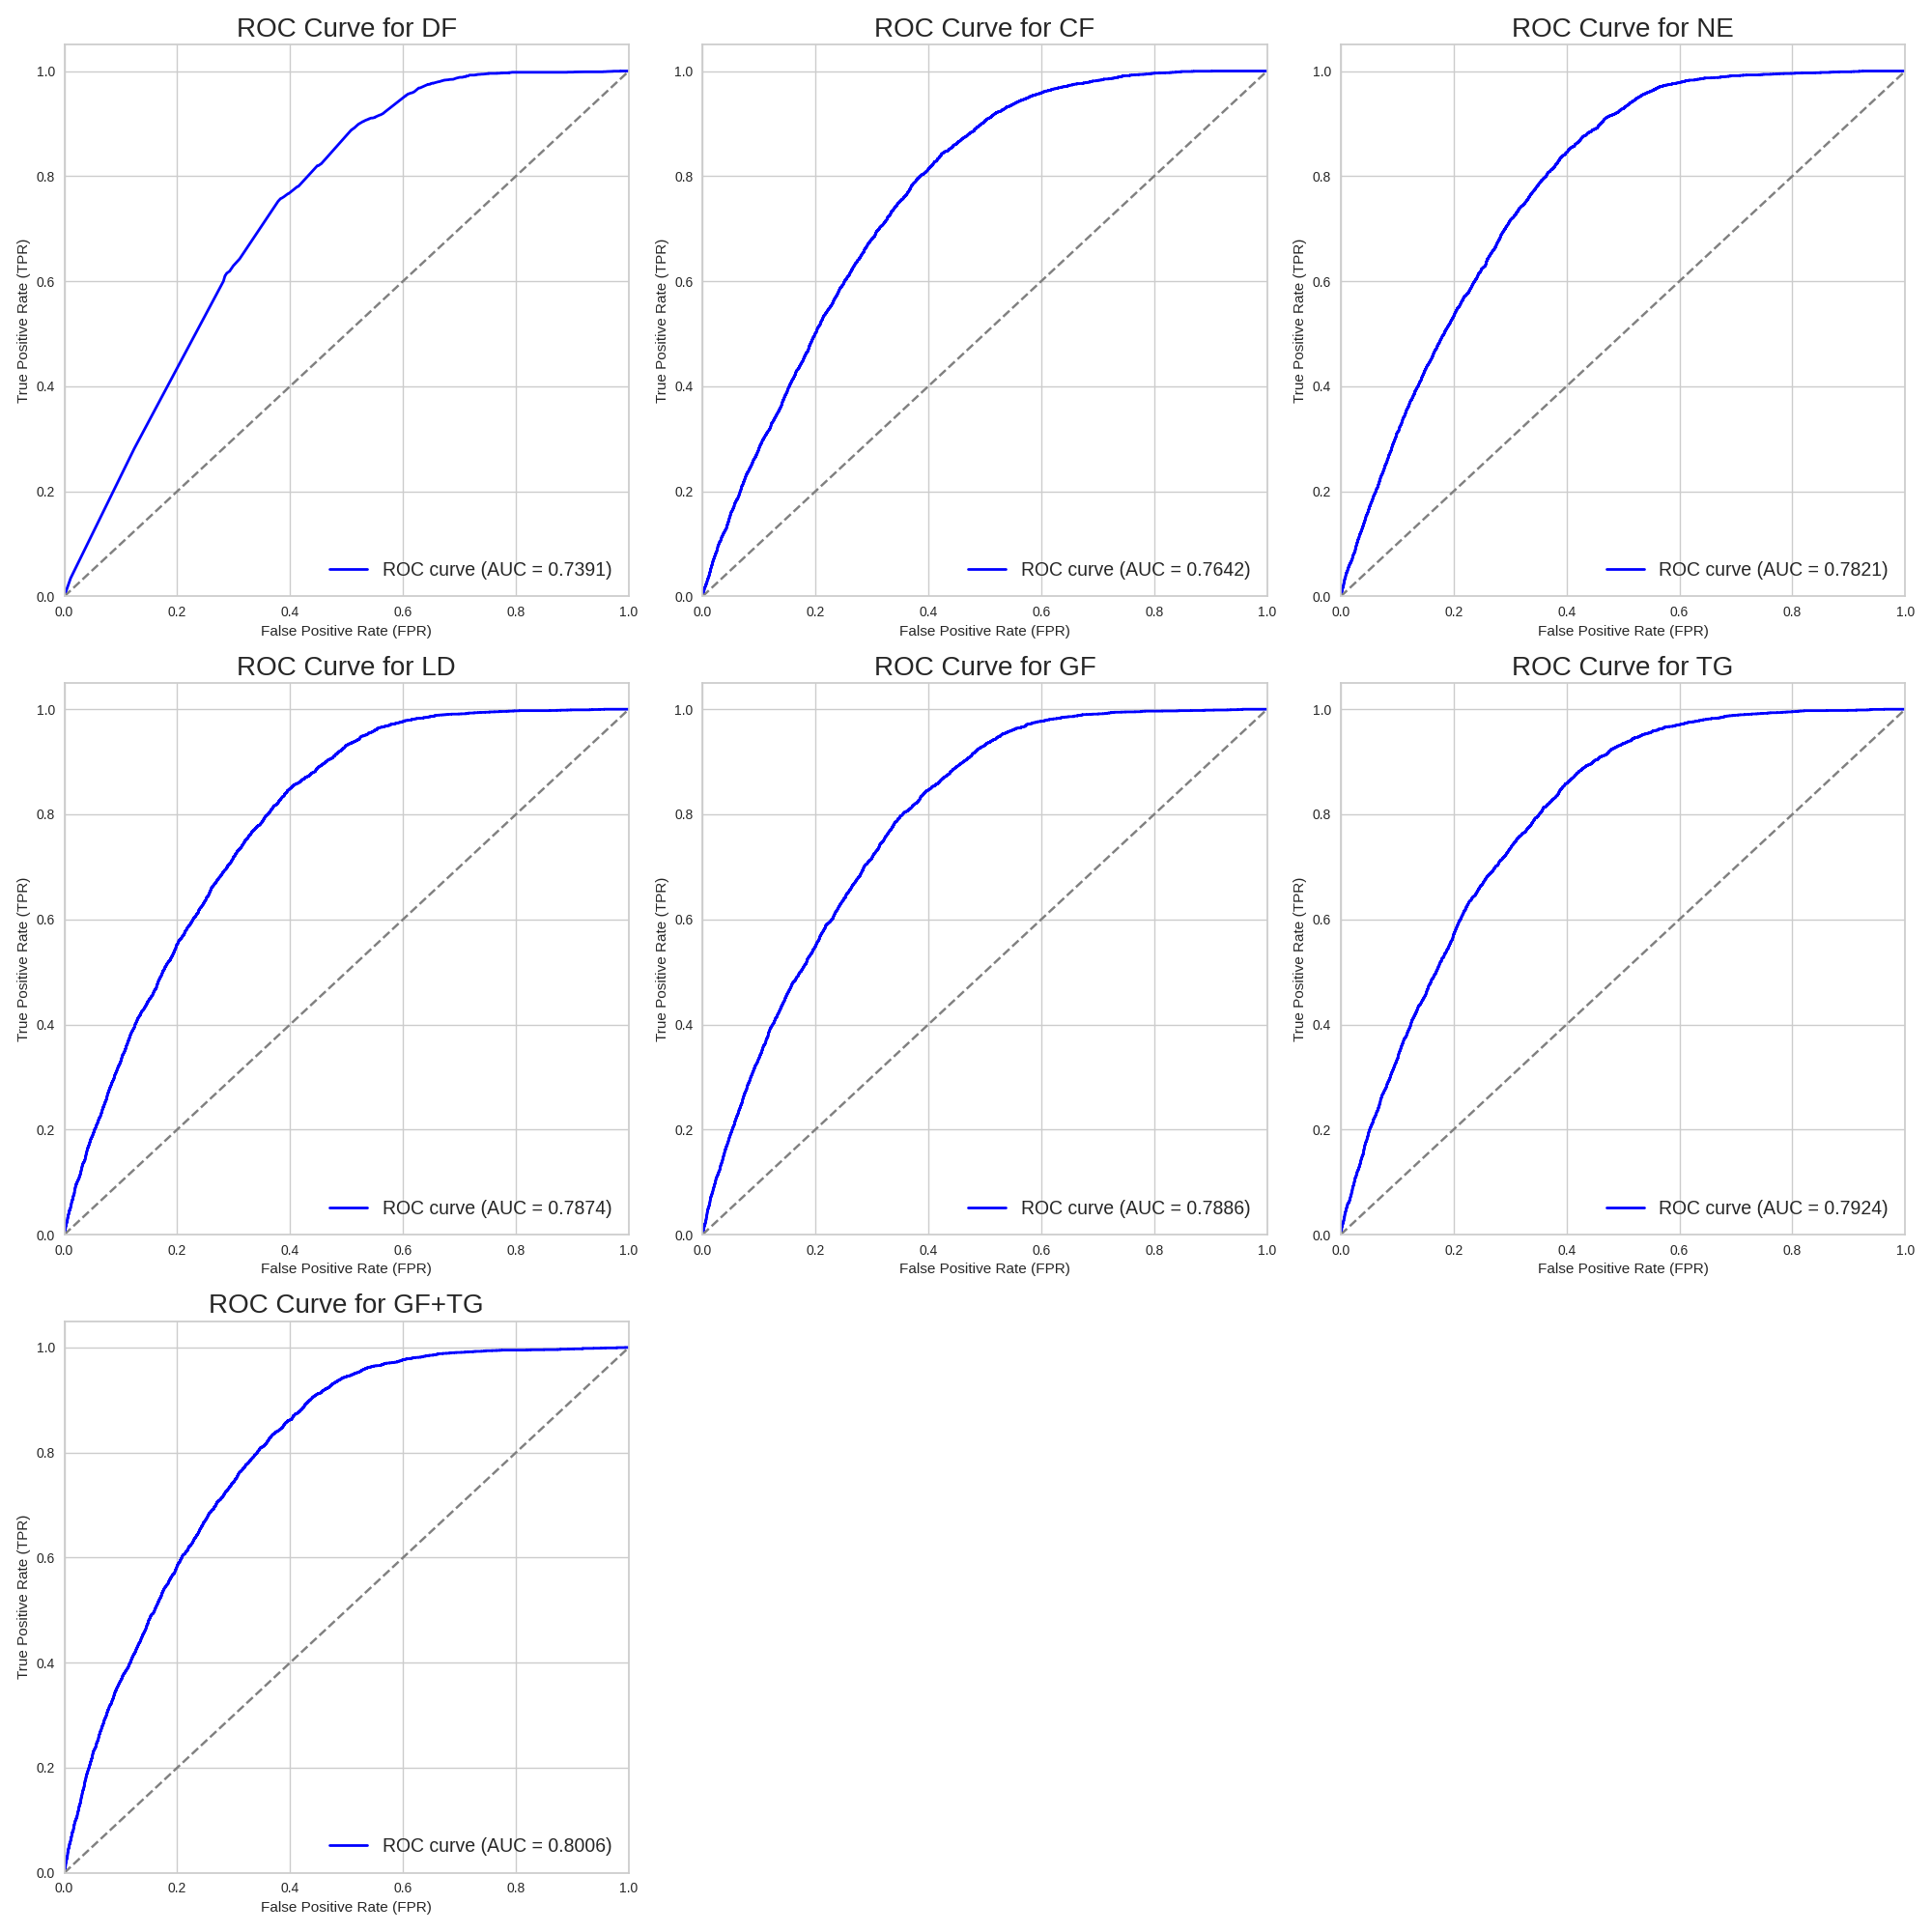
\includegraphics[scale=0.25]{./non-crime-timeseries-fig/roc_auc.png}
%   \caption{ROC曲線}
%   \label{fig:non-crime-timeseries-roc}
% \end{figure}
%------------------------------------------
% table
%------------------------------------------
各モデルの予測精度を精度指標を基に比較した結果を表\ref{tb:fig:non-crime-timeseries-index}にまとめる.
最も的中率が高いモデルはDFであるが,これは偽陽性を評価できていないのでPAIとAUCに注目する.
PAIは,DFとCFの比較から特徴量を連続化すると大きく改善し,
犯罪特徴量を追加する(CI)と更に改善することが確認できた.
またAUCは,CF・CIで同等の改善が確認できた.
% また,距離特徴量を変換するNE,LD,GF,TGではCFより改善がみられ,
% GF+TGが最もPAIが高くなった.
% AUCについて注目すると,DFとCFを比較すると精度の改善がみられた.
% LD,GF,TGでは同等の精度の改善が確認され,
% PAIと同様にGF+TGが最もAUCが高くなった.

また,DFとCIのAUC値の有意差を評価するためにDeLong検定\cite{DeLong}を実施した結果,
$p<0.001$となり,両者のAUCに統計的に有意な差があることが確認できた.

\begin{table}[htbp]
  \centering
  \caption{各モデル間の精度比較}
  \begin{tabular}{l|r||r|r}
  \hline

  モデル & DF & CF & CI \\  \hline\hline
  的中率 & \bf{57.2} & 30.2 & 31.3  \\ 
  PAI & 1.84 & 2.18 & \bf{2.29} \\ 
  AUC & 0.74 & \bf{0.76} & \bf{0.76} \\ \hline
  


  \end{tabular}
  \label{tb:fig:non-crime-timeseries-index}
\end{table}

\FloatBarrier